\documentclass{article}
\usepackage[utf8]{inputenc}
\usepackage{amsmath}
\usepackage{graphicx}
\usepackage{amssymb}
\usepackage{subcaption}
\usepackage{placeins}
\usepackage{url}
\usepackage[a4paper, margin=0.8in]{geometry}

\title{What is the best performing sorting algorithm? \\ \large Experimental analysis commissioned by Bubble Inc}
\author{Ghilardini Matteo, Toscano Sasha}
\date{\today}

\begin{document}

\maketitle

\section*{Abstract}
    In this document, we analyze and compare the performance of four sorting algorithms implemented in Java in order to determine which one represents the optimal choice in terms of efficiency and speed for the implementation of a utility function within a Bubble Inc. library.
    
    We measured and analyzed the sorting speeds of BubbleSortUntilNoChange, BubbleSortWhileNeeded, QuickSortGPT, and SelectionSortGPT in various scenarios by modifying the size, data type, and initial order of the dataset.
    
    To ensure a good level of reliability in our analysis, we repeated the sorting process multiple times for each combination of independent variables.
    
    The performance, i.e., the sorting time of each algorithm, was measured in nanoseconds using the Java function System.nanoTime().
    
    The collected data show that the QuickSortGPT algorithm offers the best performance on randomly filled datasets, which is the most common scenario in which sorting will be required. This is due to its Average Time Complexity of $O(n \log n)$.
    
    We also noticed that SelectionSortGPT and both implementations of BubbleSort have scenarios where their performance is better than that of QuickSortGPT, but these are very remote scenarios that are extremely unlikely to occur in the real world.
    

\section{Introduction}
    In this experiment, we aim to answer an important question: \textit{Which sorting algorithm implementation in Java is most efficient?} Efficient sorting is critical in computer science because many applications rely on sorting as a fundamental operation, whether in data processing, search optimization, or user interfaces. Selecting the most effective sorting algorithm can significantly impact the performance of these applications, especially when handling large datasets. 
    
    In this study, we will analyze several Java sorting algorithm implementations with distinct characteristics: 
    \begin{itemize}
        \item BubbleSortUntilNoChange
        \item BubbleSortWhileNeeded
        \item QuickSortGPT
        \item SelectionSortGPT
    \end{itemize}
    
    To determine the best sorting performance, we will compare the algorithms by measuring the time required to sort arrays of varying sizes and data types. To enhance the reliability of our findings, we will average sorting times across multiple repetitions for each scenario.
    
    By examining the efficiency of each algorithm in this way, we hope to provide insights into which implementation is most suitable for different use cases.
    
    \subsection*{Hypothesis}
    The QuickSort algorithm is the best one in terms of performance since its complexity is $O(n*logn)$; compared to BubbleSort $O(n^2)$ and Selection Sort $O(n^2)$. 
    
    We expect this behavior for every data type, array size and starting array order.

\newpage
    
\section{Method}
    \subsection{Variables}
    \begin{table}[h!]
        \centering
        \begin{tabular}{l|c|l}
            \textbf{Independent variable} & \textbf{Levels} & \textbf{Description} \\ \hline
            Different algorithms & 4 & 4 different algorithms \\ 
            Data types & 3 & Integer (4 bytes), Char (2 bytes), Boolean (1 bit) \\ 
            Size of the array & 2 & Integer number, we selected 1,000 and 10,000 \\ 
            Starting array order & 3 & Sorted, Shuffled, or Reverse-sorted \\
        \end{tabular}
        \caption{Independent variables}
    \end{table}

    \begin{table}[h!]
        \centering
        \begin{tabular}{l|c|l}
            \textbf{Dependent variable} & \textbf{Measurement scale} & \textbf{Measurement method} \\ 
            \hline
            Time to complete the sorting & nanoseconds & \texttt{System.nanoTime()} \\
        \end{tabular}
        \caption{Dependent variables}
    \end{table}

    \begin{table}[h!]
        \centering
        \begin{tabular}{l|l}
            \textbf{Control variable} & \textbf{Fixed value} \\ \hline
            Number of active applications & None outside of IDE and WSH Terminal \\
            Computer HW, OS, JDK & Intel i7-9700k, 32GB RAM, Windows 10, OpenJDK 23.01 \\ 
        \end{tabular}
        \caption{Control variables}
    \end{table}

    \FloatBarrier

    \subsection{Design}
    \subsubsection{Study Type}
        
        \begin{table}[!h]
            \centering
            \begin{tabular}{c|c|c}
                \textbf{Observational Study} & \textbf{Quasi-Experiment} & \textbf{Experiment} \\ \hline
                \(\square\) & \(\square\) & \(\boxtimes\) \\
            \end{tabular}
            \caption{Study type selection}
        \end{table}

        We are conducting an \textbf{experiment} because we are actively \textit{manipulating the independent variables} (i.e., we observe how performance changes with different sorting algorithms, data types, array sizes, and initial orders). This manipulation allows us to examine cause-and-effect relationships between these variables and the time taken to sort.

        Additionally, we are using \textbf{randomization} in our experimental design. The data used to populate the arrays for each trial are generated randomly, ensuring that each algorithm operates on arrays that are equivalent in content and structure for a given data type and size. This helps balance out any potential biases or differences, as each algorithm sorts the same sets of data under comparable conditions.
        
        We also have \textbf{control conditions}, where we can compare each algorithm's performance as a benchmark or "status quo" against others within the same experimental conditions. This allows us to determine if certain algorithms outperform others or if the effects vary based on the data characteristics.

    \subsubsection{Number of Factors}
        \begin{table}[!h]
            \centering
            \begin{tabular}{c|c|c}
                \textbf{Single-Factor Design} & \textbf{Multi-Factor Design} & \textbf{Other} \\ \hline
                \(\square\) & \(\boxtimes\) & \(\square\) \\
            \end{tabular}
            \caption{Number of factors selection}
        \end{table}

        Our experiment uses a \textbf{Multi-Factor Design} since we are manipulating multiple \textit{independent variables} to observe their effect on the dependent variable, the sorting time. \\ 
        This design allows us to observe the effect of all independent variables on the dependent variable. \\
        By analyzing all combinations, we are performing a \textit{Full factorial design} resulting in: 
        \[
        \#\text{algorithms} \times \#\text{dataTypes} \times \#\text{sizes} \times \#\text{startingOrders} = 4 \times 3 \times 2 \times 3 = 72 \text{ different results}
        \]
        
        To visualize this concept, we can imagine it as a flowchart diagram, where each dependent variable is a state with \( n \) possible outcomes from it. As follows (to avoid drawing all 72 possible paths, we have simplified the drawing by following the path of \textit{QuickSortGPT, 1'000, Random, ...}):

        \begin{figure}[!h]
            \centering
            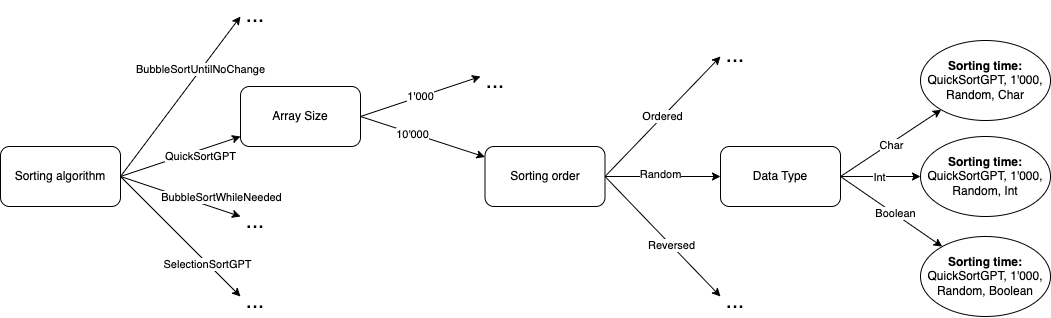
\includegraphics[width=1\linewidth]{MultiFactorDesign.png}
            \caption{Multi-Factor Design}
            \label{fig:multifactorDesign}
        \end{figure}

        \FloatBarrier

    \subsection{Apparatus and Materials}
        We will run all experiments on a desktop computer with the following hardware specifications:
        \begin{itemize}
            \item \textbf{CPU:} Intel Core i7-9700k
            \item \textbf{RAM:} 32GB DDR4
        \end{itemize}
        
        The computer runs on Windows 10 as the operating system, but all experiments and the JDK are executed through the WSL with Ubuntu 23.04.
        
        We are using OpenJDK 23.01 as the Java version and as IDE we used Microsoft VSCode. For all experiments performed, we save all metrics in a CSV file, and to plot the data, we use Microsoft Excel 365.
        
        To measure the metrics of the experiments, we use the Java function \texttt{System.nanoTime()} and save the value before and after sorting. The elapsed time is then computed as \texttt{startTime - endTime}.

    \subsection{Procedure}
        The procedure for running the experiment begins by restarting the PC (so as to make sure there are no background applications running). When the machine is restarted, we start only the IDE (VSCode) and the WSL terminal. At this point we execute our code.
        
        We have implemented a function \texttt{runTests(repetitions, arraySize)}, and we call it from the \texttt{Main} method 3 times:
        \begin{itemize}
            \item \texttt{runTests(10, 1000)} is a warm-up run, so we only need a few iterations on an array of discrete size
            \item \texttt{runTests(100, 1000)}
            \item \texttt{runTests(100, 10000)}
        \end{itemize}

        We opted to choose 10 repetitions of an array of size 1'000 as a valid warm up as during our testings we saw that most of the data stabilized after roughly 2-5 iterations. So we accounted for the worst-case scenario and added some extra margin to prevent possible outliers. We also saved that data in different files \textit{(results/warmup*)} to be able to compare it and make sure that there was still a significant difference in the results. And as we can see from comparing the results from table \ref{fig:avg1000sort} and the results of the warm up averages (which can be seen in figure \ref{fig:warmup_avg_1000_random}) there is about a 30\% difference in all averages.

        The function \texttt{runTests(...)} sets up the environment for the testing; it creates all the arrays of different types (int, char, boolean) and different orders (random, sorted, reverse-sorted) with the corresponding functions, and sets the path of all the CSV files where we will save the results. After that, we call the function \texttt{performSortingTests(...)} that is responsible to measure and save the results of all sorting algorithms.

        The function \texttt{performSortingTests(...)} runs all sorting algorithms for the given combination of independent variables, and stores the resulting data and the average sorting time in a specific CSV file.

\newpage
        
\section{Results}
    \subsection{Visual Overview}
    In the visual overview we have chosen to report graphs representing the average sorting times of the various algorithms. We have chosen to keep the graph for the randomly filled arrays larger, and therefore more visible, since it represents the “average case” for which our library will be used.
    
    As an appendix to the paper, however, graphs representing the sorting times of each combination of the independent variables for each of the 100 repetitions performed are also shown in chapter \ref{chap:appendix}. In these graphs it can be easily seen that the performance of each sorting algorithm tends to be smooth with only a few outliers.
    
    \begin{figure}[!h]
        \centering
        \begin{subfigure}{0.7\textwidth}
            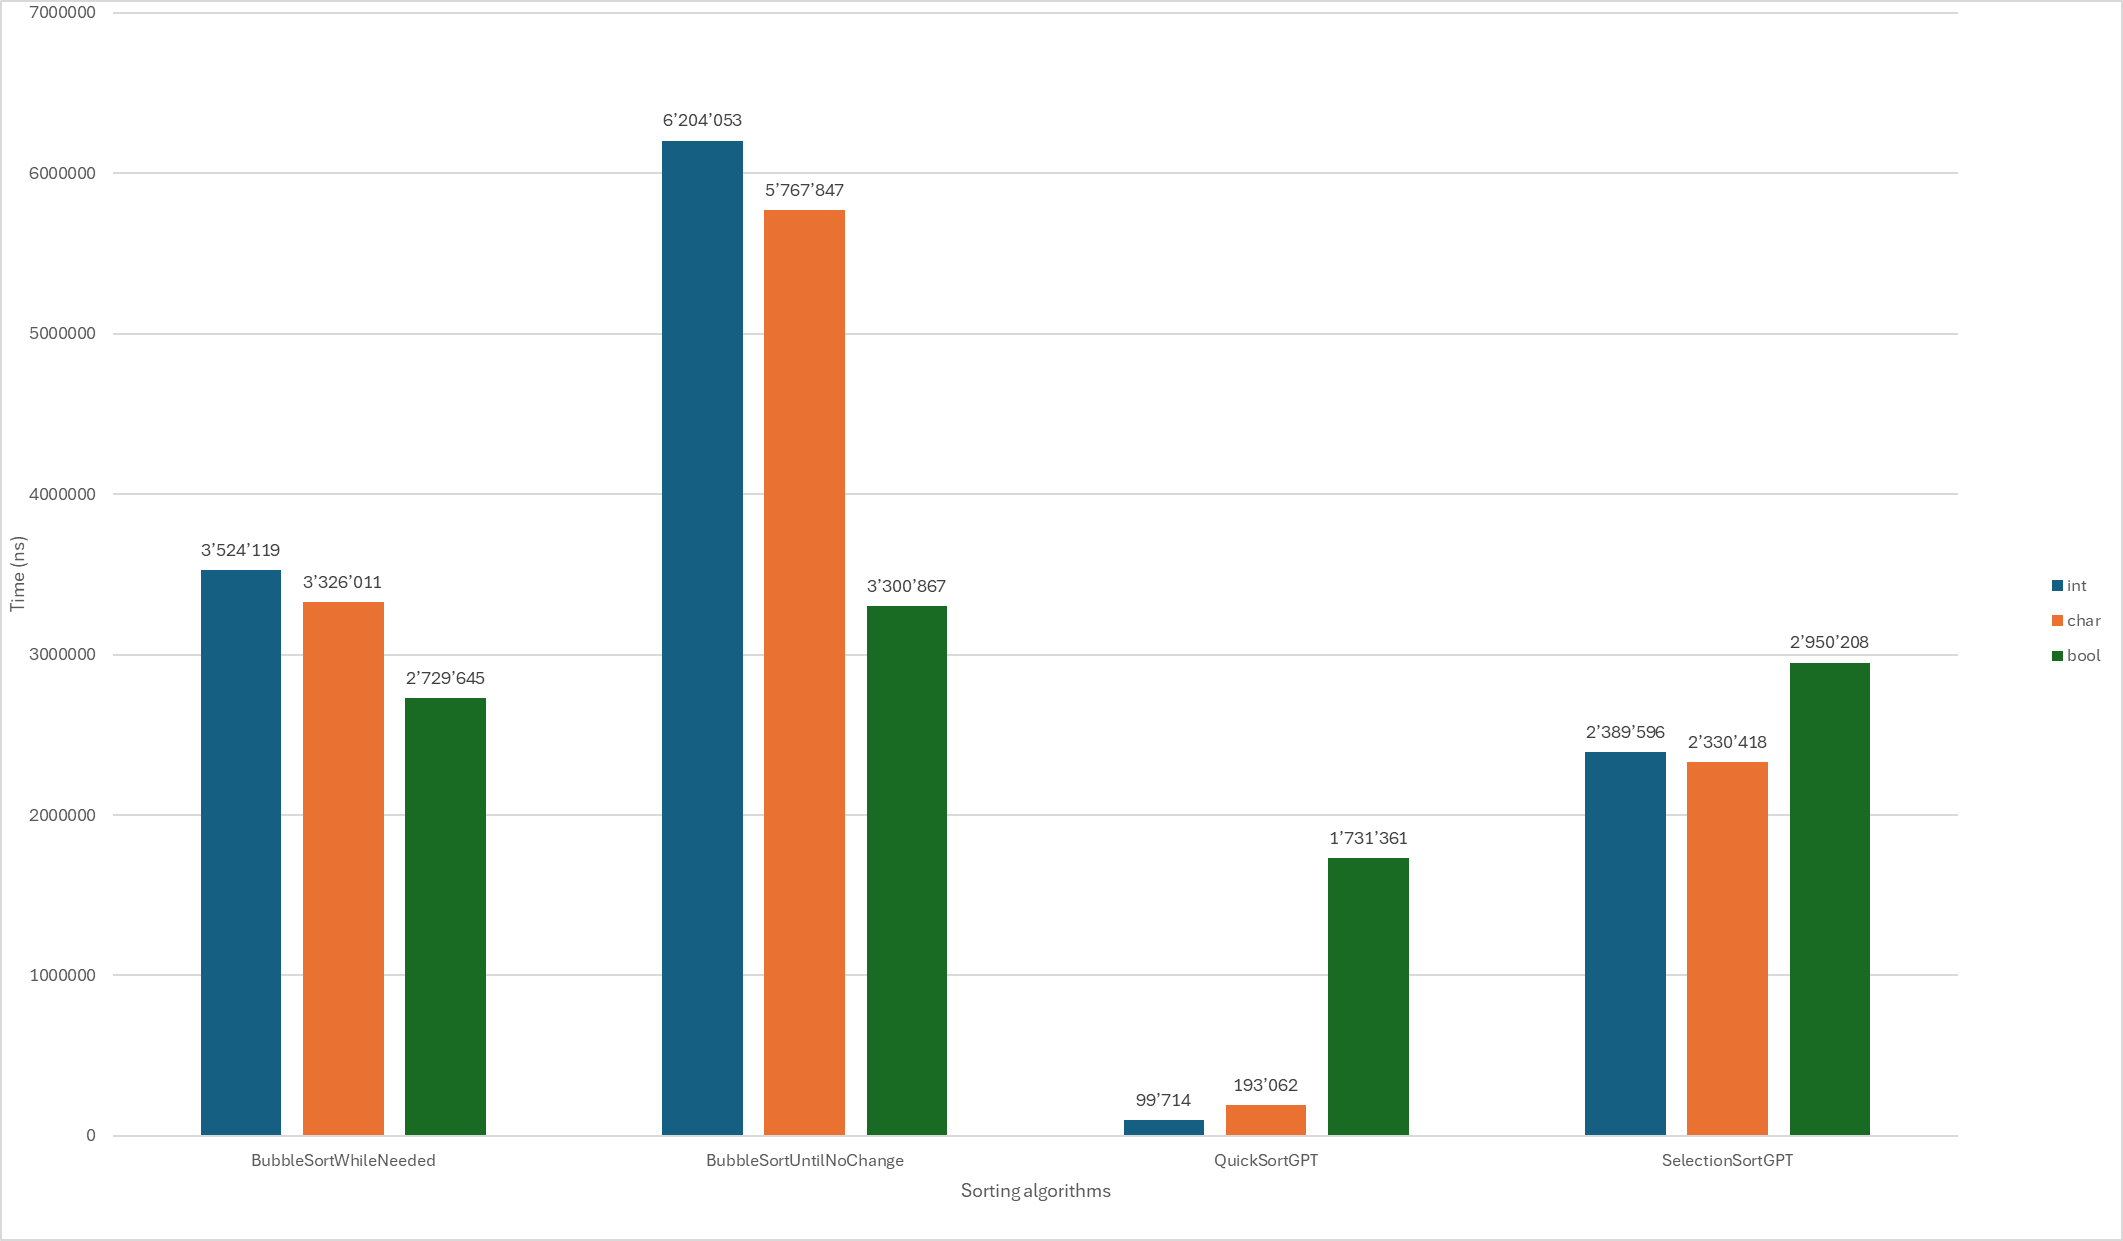
\includegraphics[width=1\linewidth]{avg1000rand.png}
            \caption{Random filled array}
            \label{fig:avg1000sort}
        \end{subfigure}
        \begin{subfigure}{0.45\textwidth}
            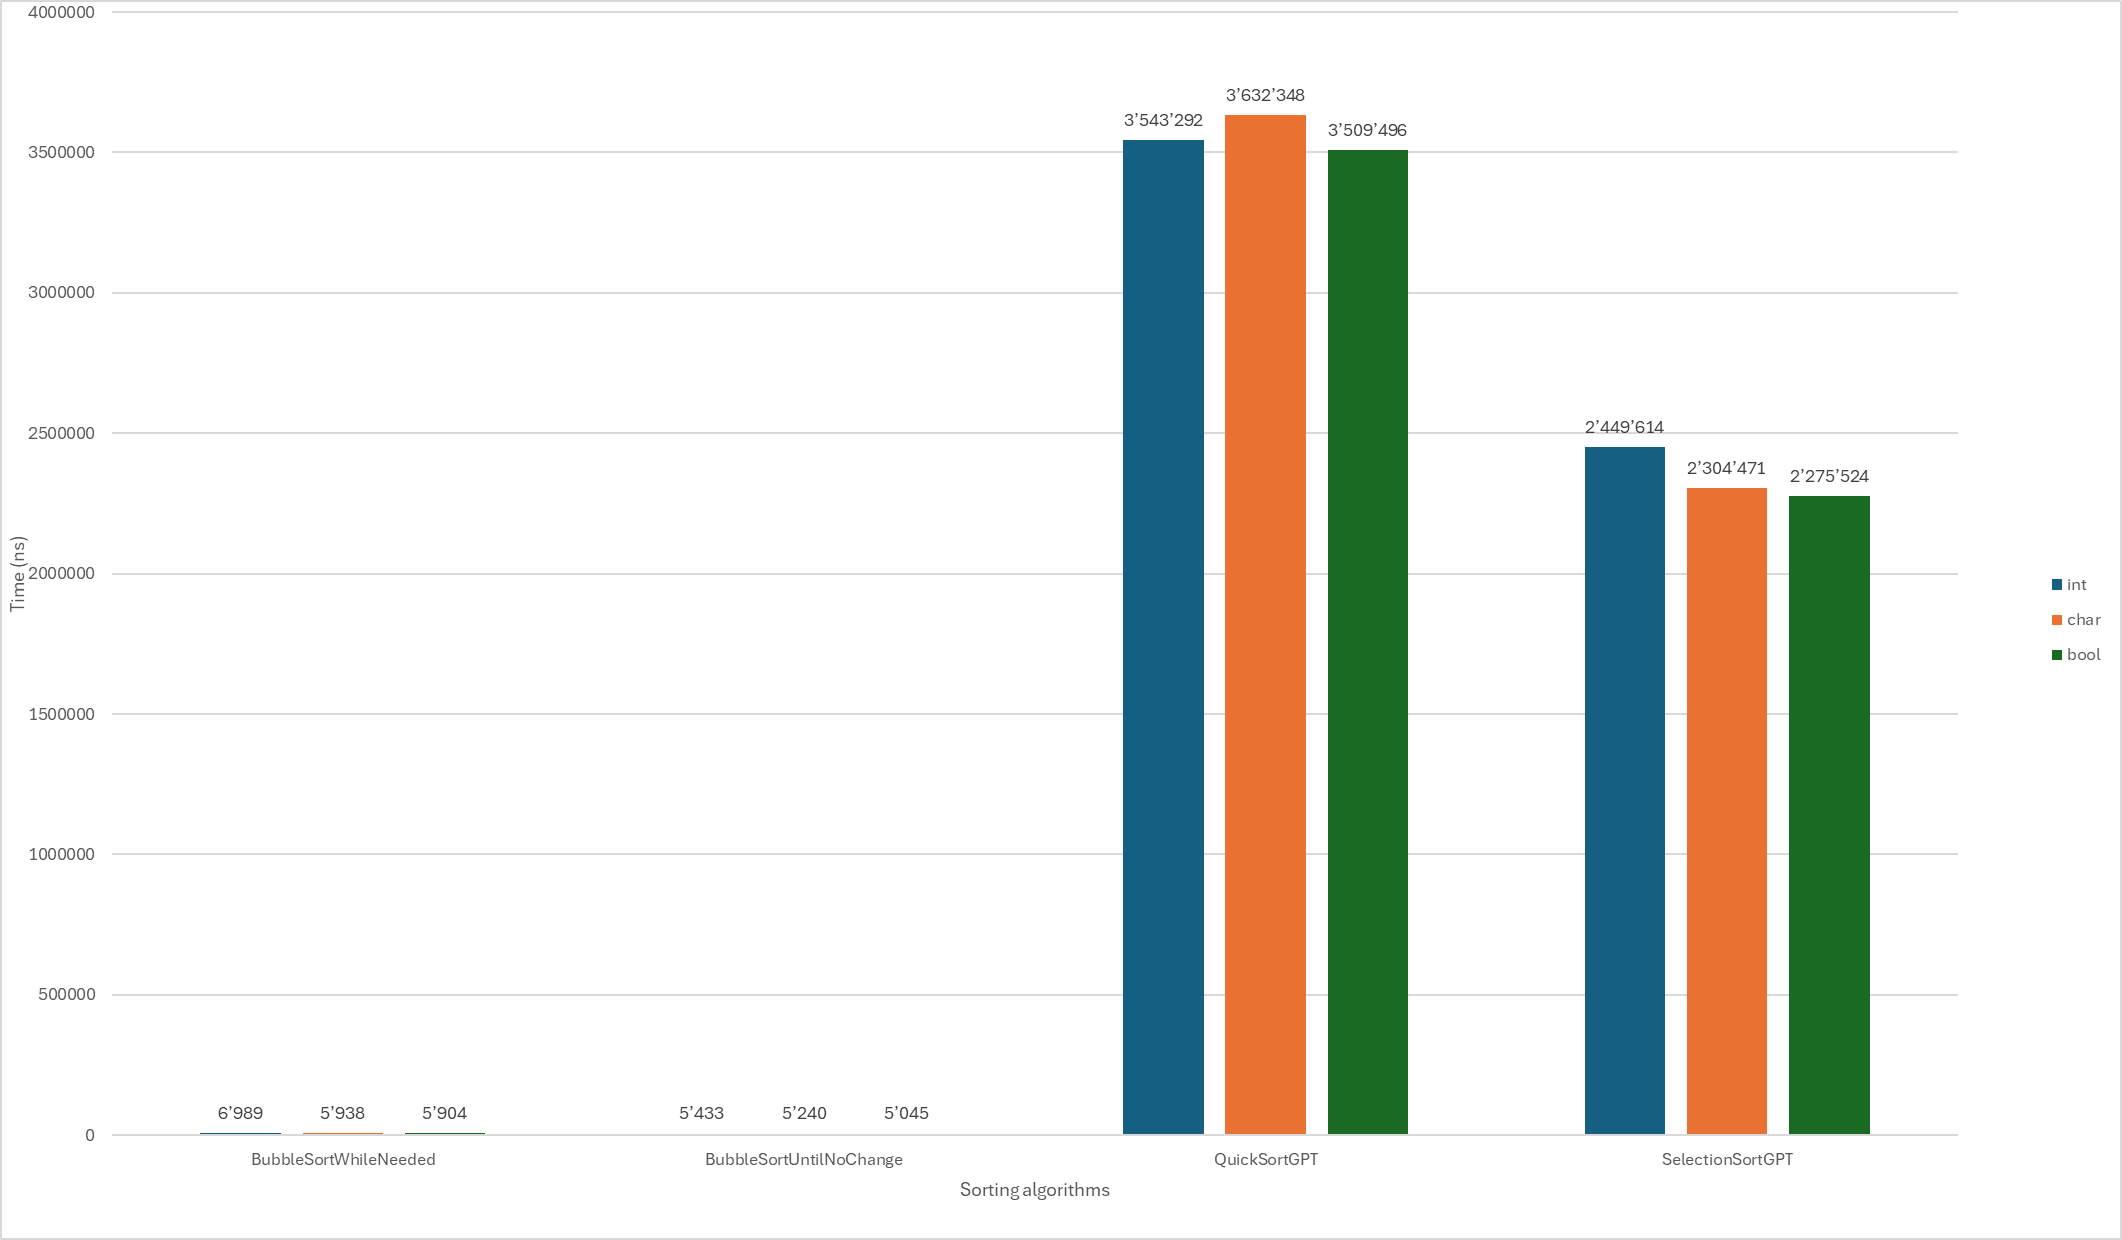
\includegraphics[width=1\linewidth]{avg1000sort.png}
            \caption{Sorted array}
            \label{fig:avg1000sort}
        \end{subfigure}
        \hfill
        \begin{subfigure}{0.45\textwidth}
            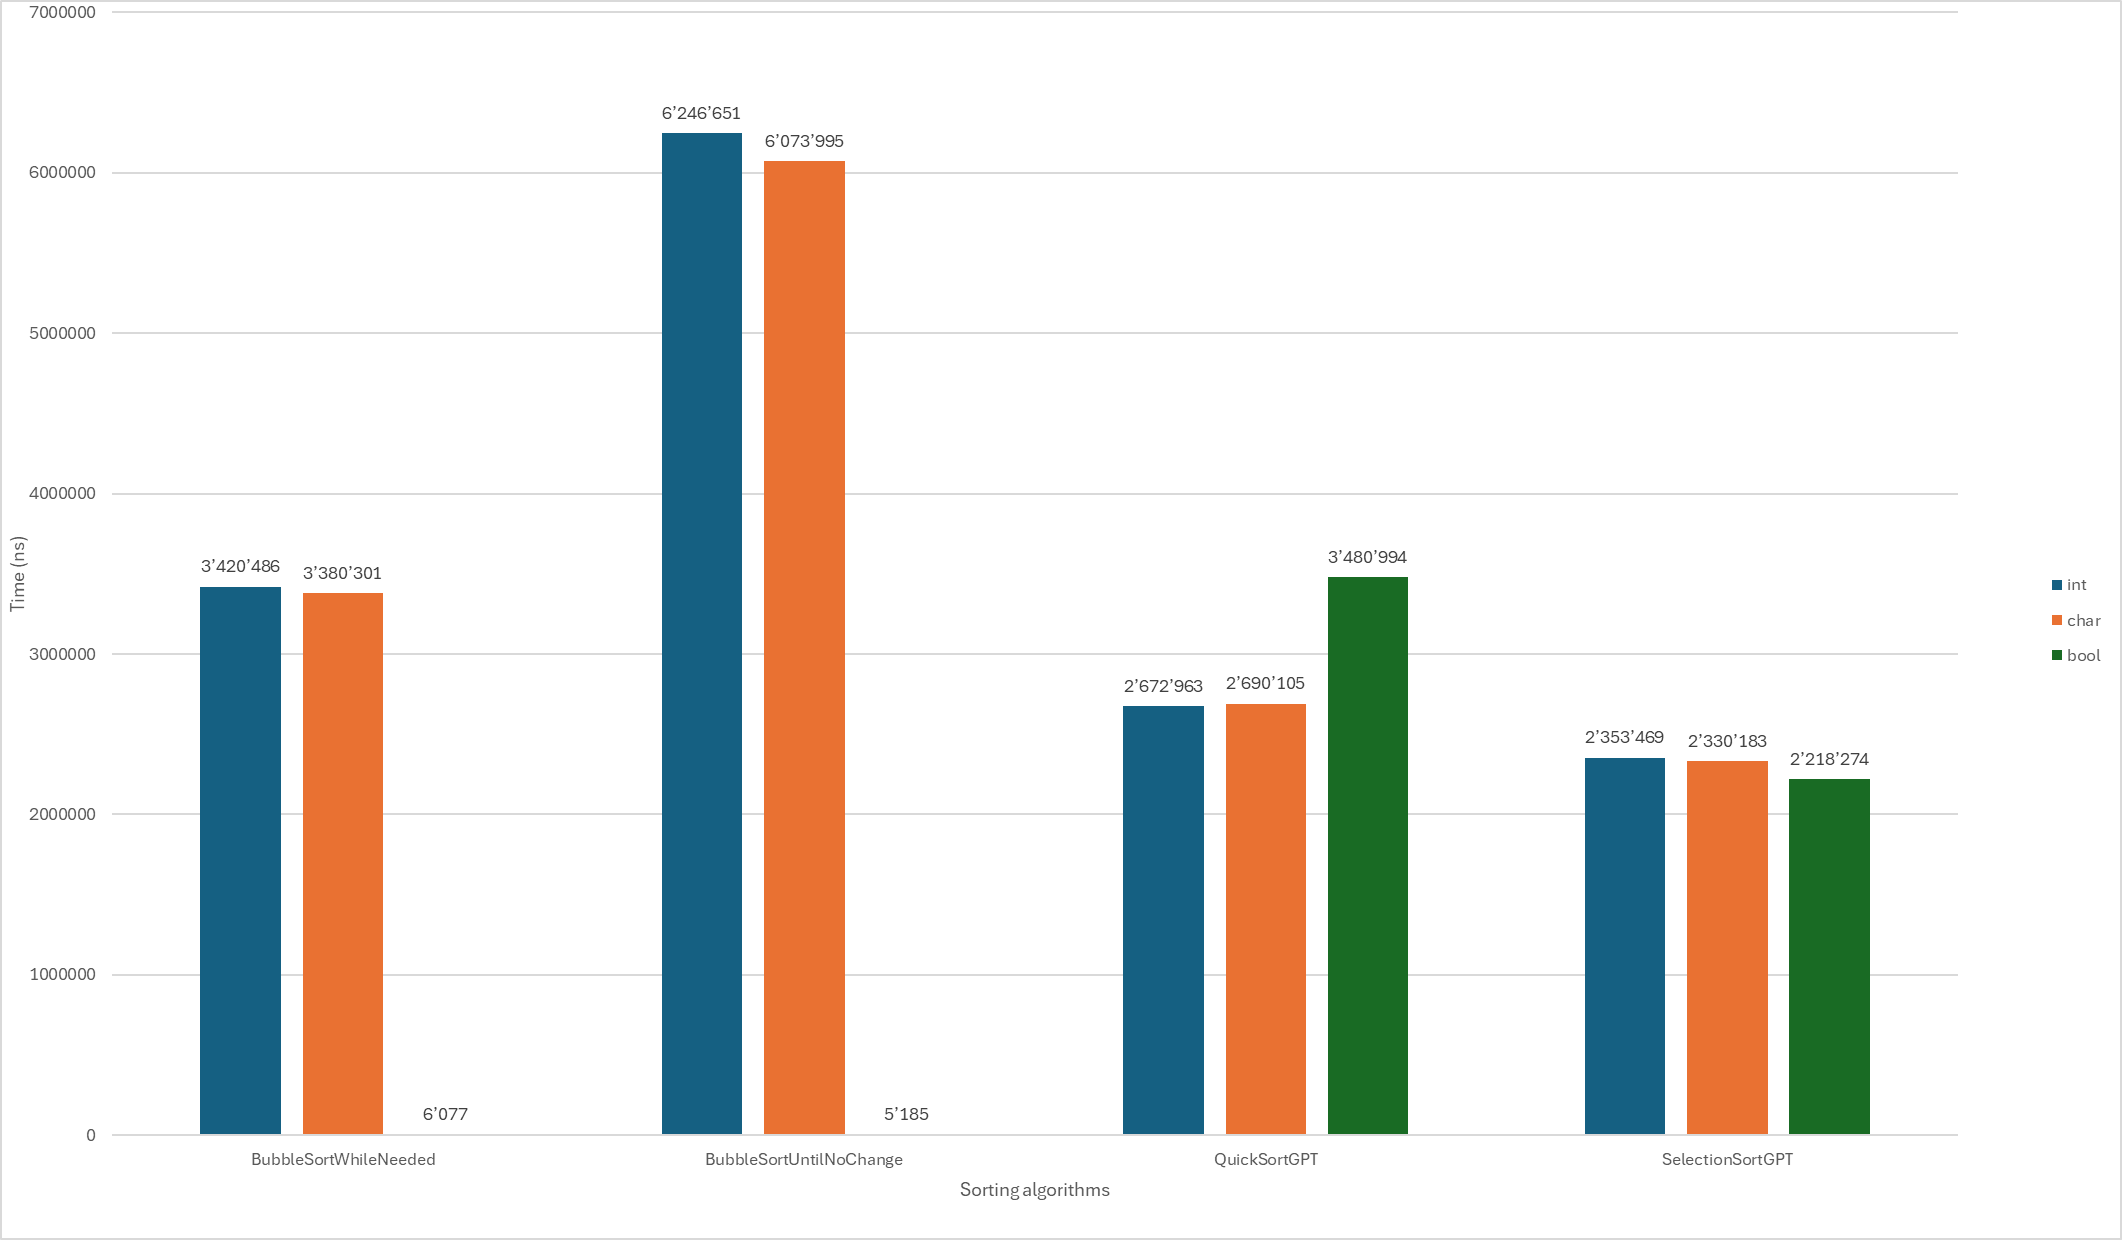
\includegraphics[width=1\linewidth]{avg1000rev.png}
            \caption{Reverse sorted}
            \label{fig:avg1000rev}
        \end{subfigure}
        \caption{Average sorting time - 1000}
        \label{fig:avg1000}
    \end{figure}
    
    \begin{figure}[!h]
        \centering
        \begin{subfigure}{0.7\textwidth}
            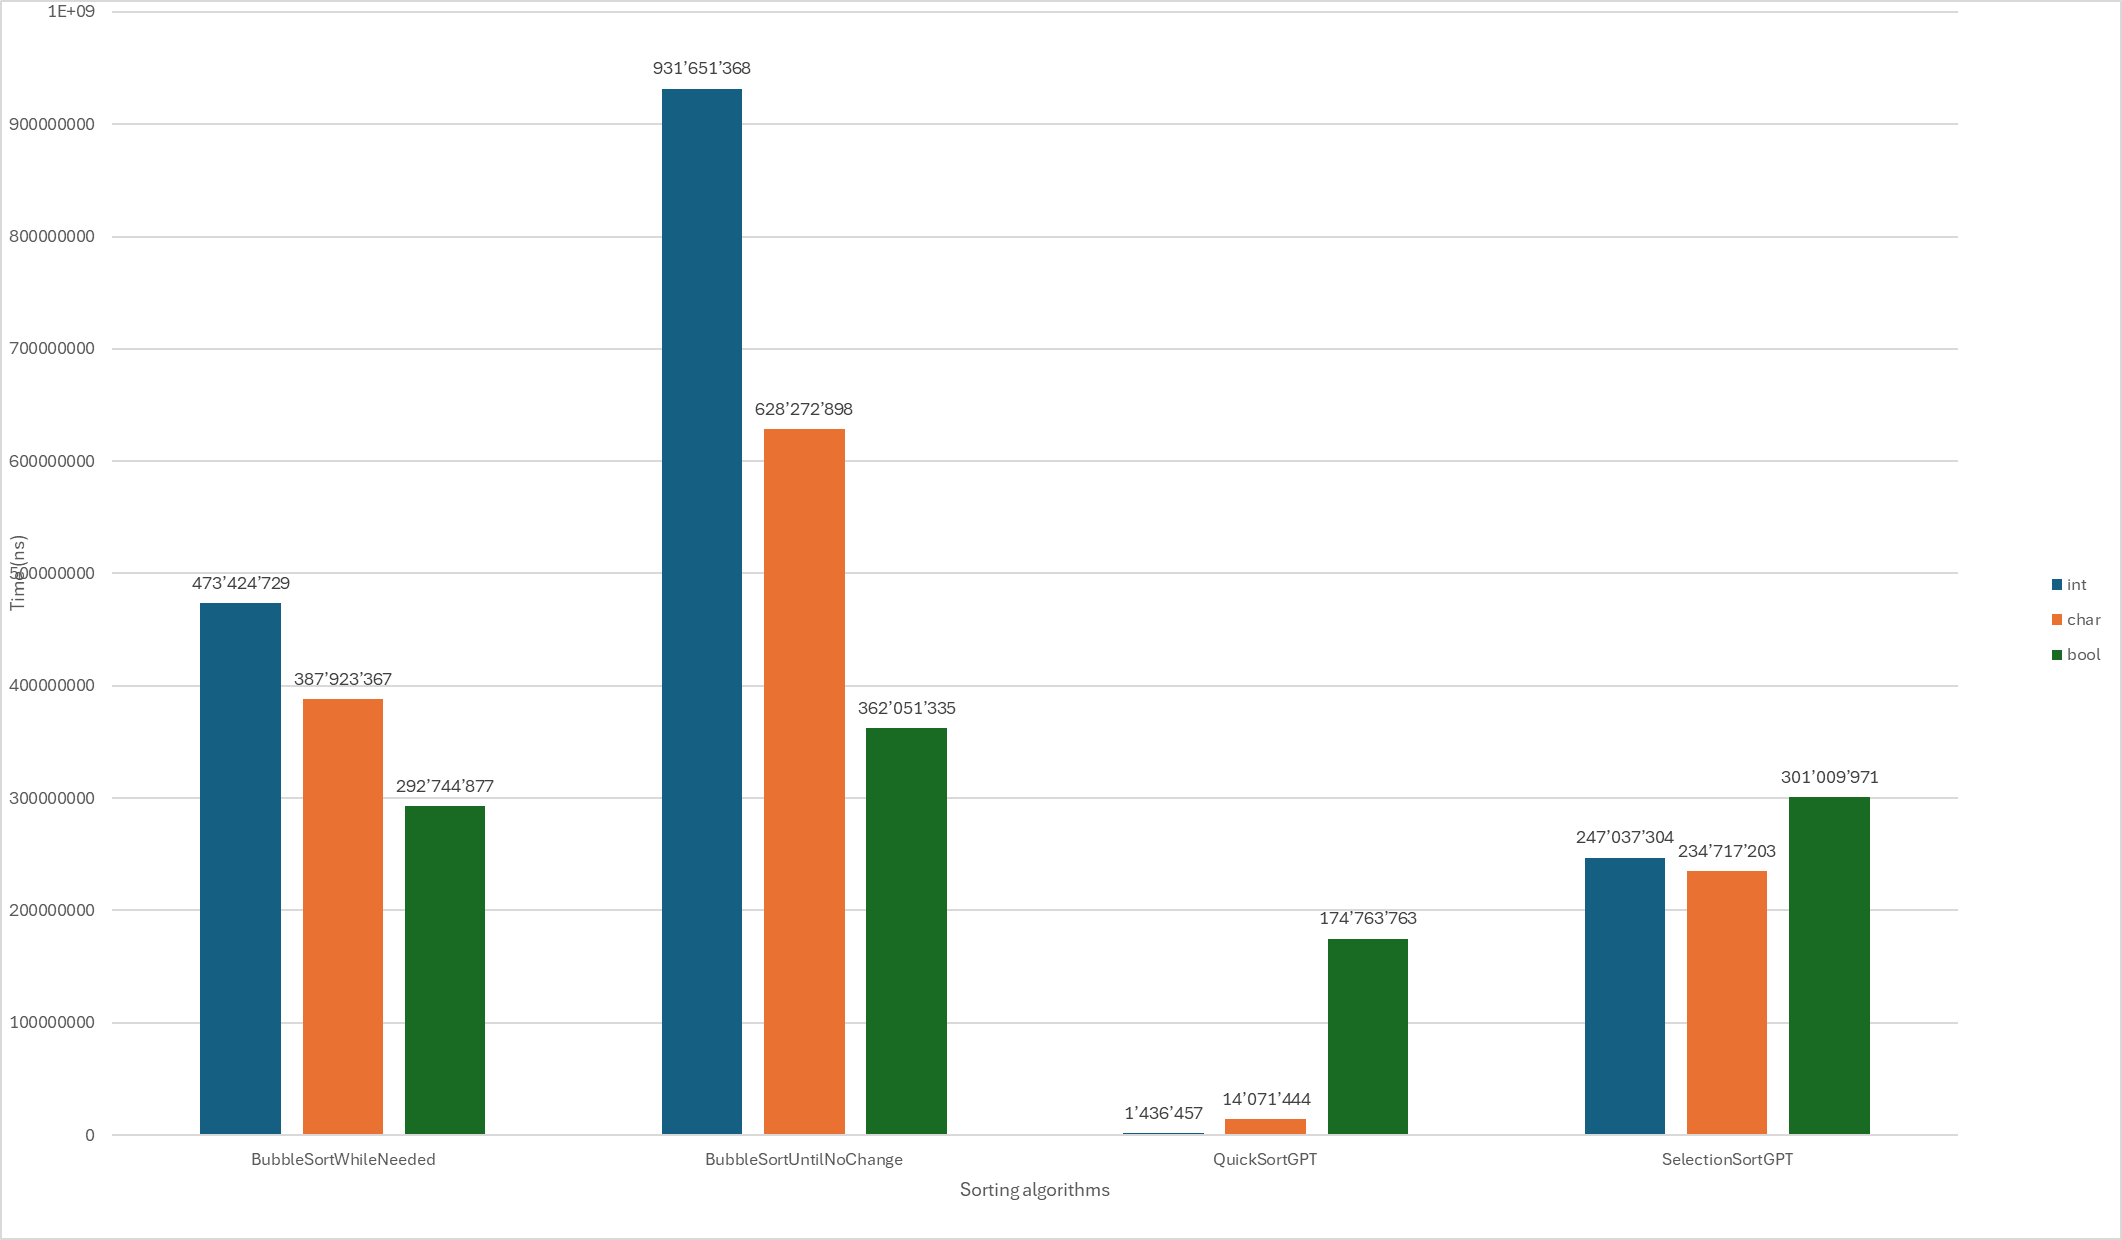
\includegraphics[width=1\linewidth]{avg10000rand.png}
            \caption{Random filled array}
            \label{fig:avg10000sort}
        \end{subfigure}
        \begin{subfigure}{0.45\textwidth}
            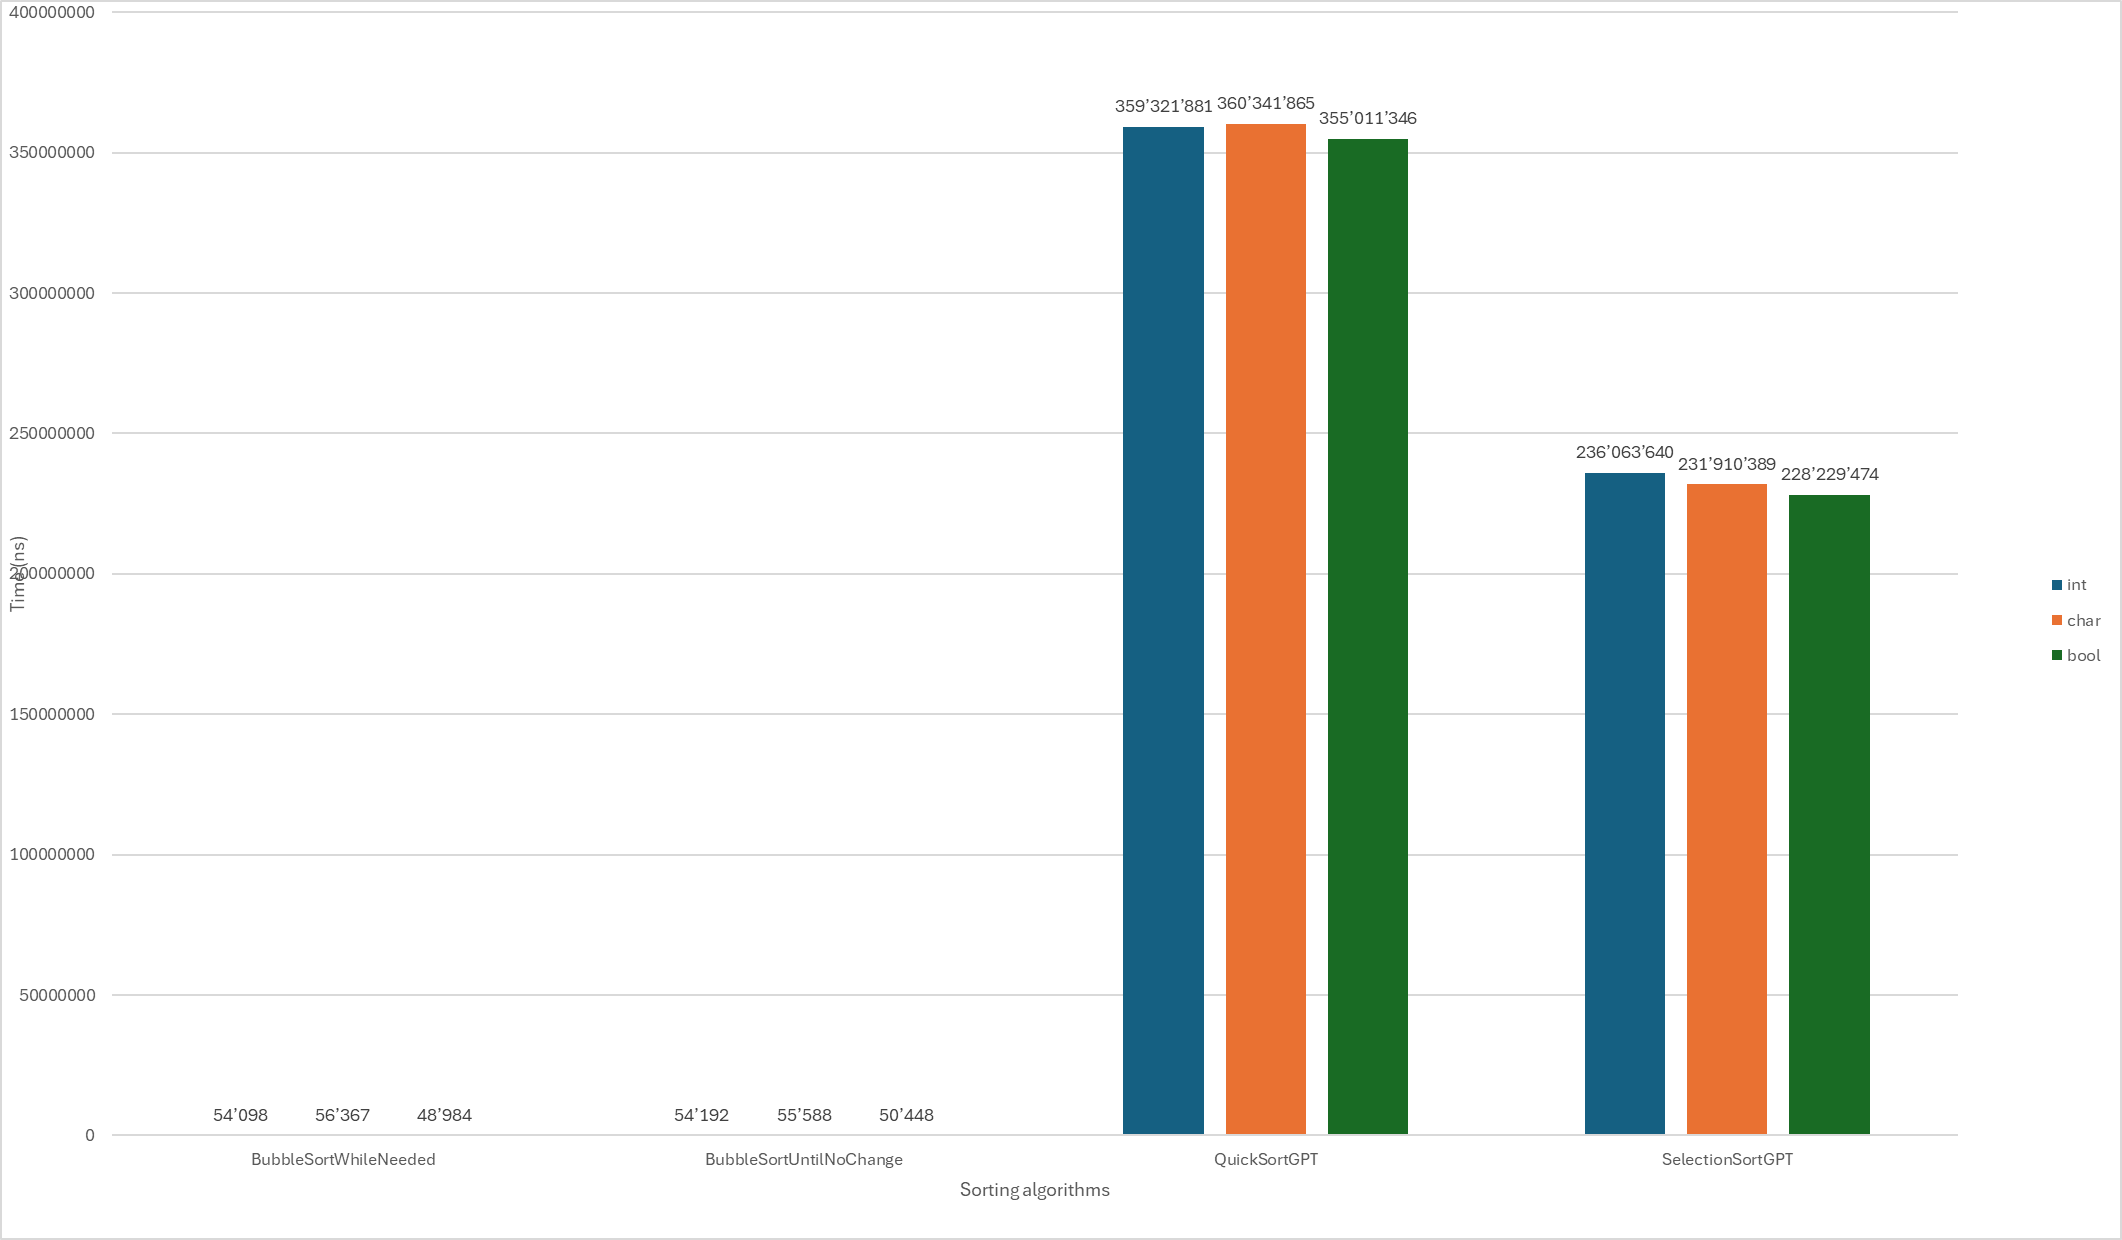
\includegraphics[width=1\linewidth]{avg10000sort.png}
            \caption{Sorted array}
            \label{fig:avg10000sort}
        \end{subfigure}
        \hfill
        \begin{subfigure}{0.45\textwidth}
            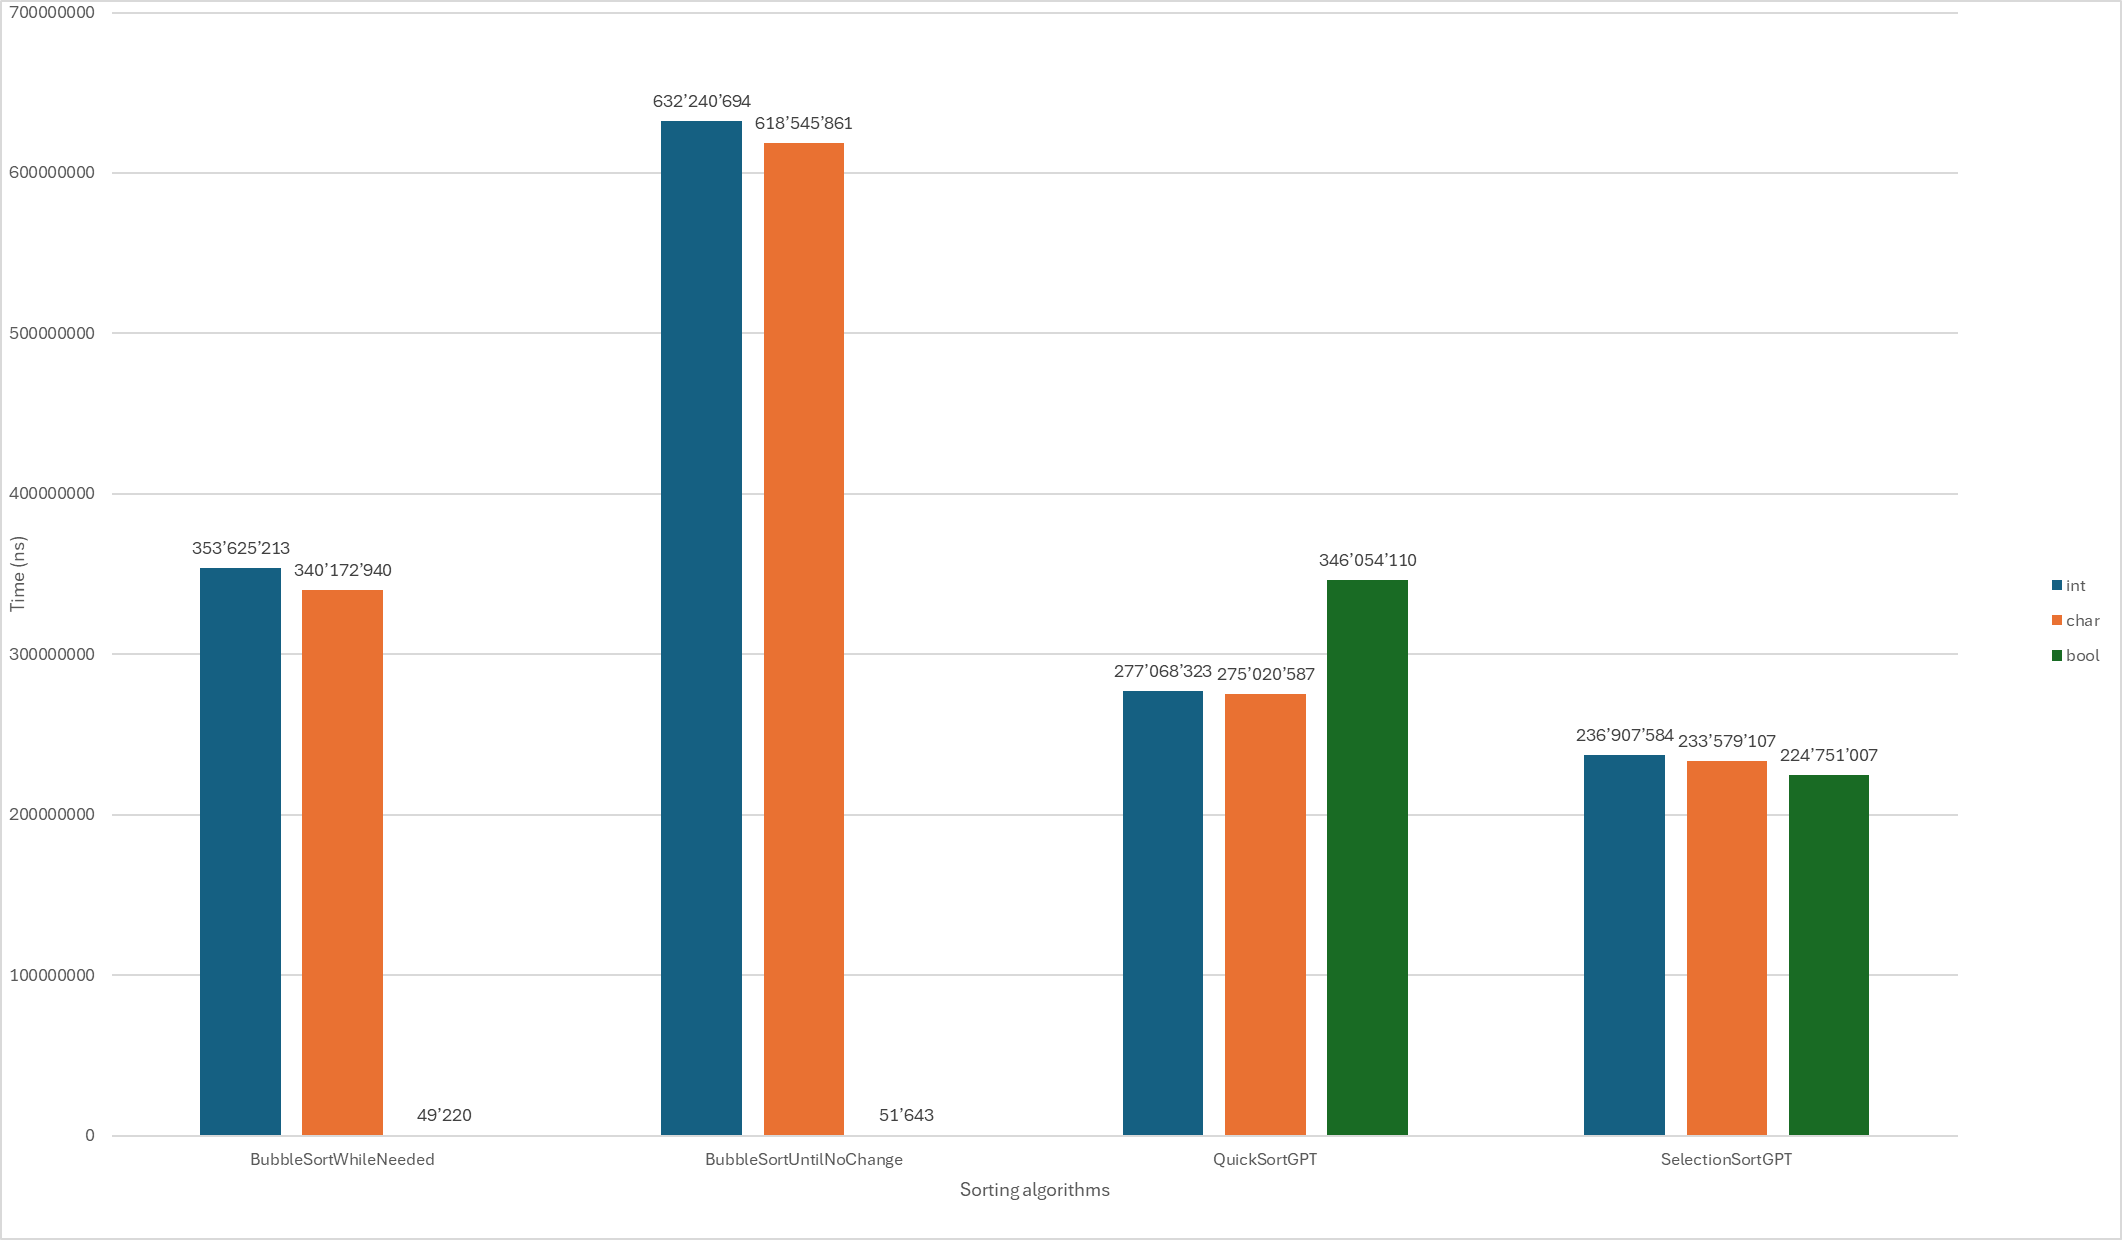
\includegraphics[width=1\linewidth]{avg10000rev.png}
            \caption{Reverse sorted}
            \label{fig:avg10000rev}
        \end{subfigure}
        \caption{Average sorting time - 10'000}
        \label{fig:avg10000}
    \end{figure}

    \FloatBarrier

    \subsection{Descriptive Statistics}
    In the tables below, we have reported the main statistics from our analysis. The data is formatted so that the best (the smallest) results are highlighted in green, the worst (the largest) in red, and the other data are formatted using a color gradient within the range.
    \begin{figure}[!h]
        \centering
        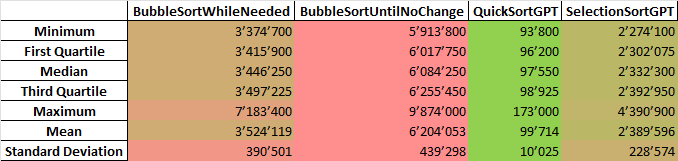
\includegraphics[width=0.75\linewidth]{int1000rand-stat.png}
        \caption{Statistics for int[1000] random filled}
        \label{fig:int1000rand-stat}
    \end{figure}
    \begin{figure}[!h]
        \centering
        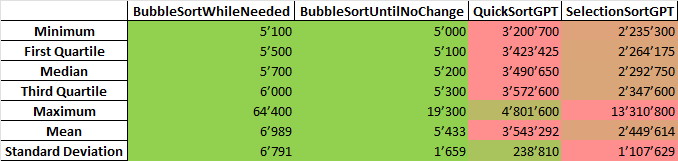
\includegraphics[width=0.75\linewidth]{int1000sort-stat.png}
        \caption{Statistics for int[1000] sorted}
        \label{fig:int1000sort-stat}
    \end{figure}
    \begin{figure}[!h]
        \centering
        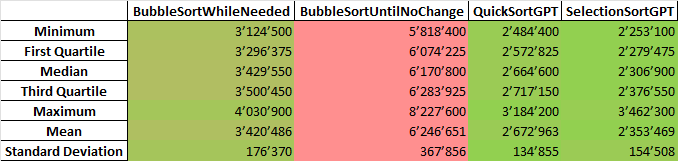
\includegraphics[width=0.75\linewidth]{int1000rev-stat.png}
        \caption{Statistics for int[1000] reverse}
        \label{fig:int1000rev-stat}
    \end{figure}
    \begin{figure}[!h]
        \centering
        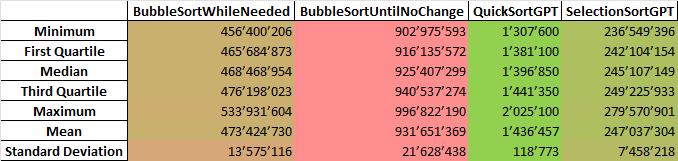
\includegraphics[width=0.75\linewidth]{int10000rand-stat.png}
        \caption{Statistics for int[10000] random filled}
        \label{fig:int10000rand-stat}
    \end{figure}
    \begin{figure}[!h]
        \centering
        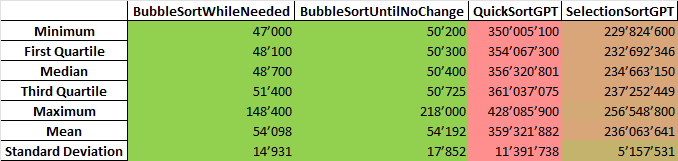
\includegraphics[width=0.75\linewidth]{int10000sort-stat.png}
        \caption{Statistics for int[10000] sorted}
        \label{fig:int10000sort-stat}
    \end{figure}
    \begin{figure}[!h]
        \centering
        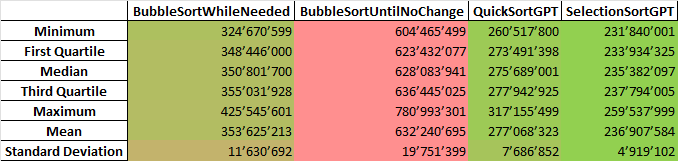
\includegraphics[width=0.75\linewidth]{int10000rev-stat.png}
        \caption{Statistics for int[10000] reverse}
        \label{fig:int10000rev-stat}
    \end{figure}
    \begin{figure}[!h]
        \centering
        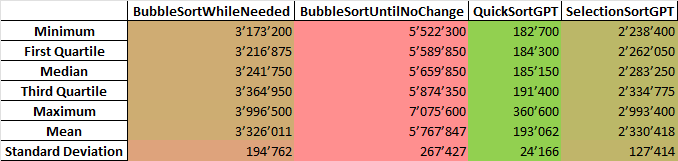
\includegraphics[width=0.75\linewidth]{char1000rand-stat.png}
        \caption{Statistics for char[1000] random filled}
        \label{fig:char1000rand-stat}
    \end{figure}
    \begin{figure}[!h]
        \centering
        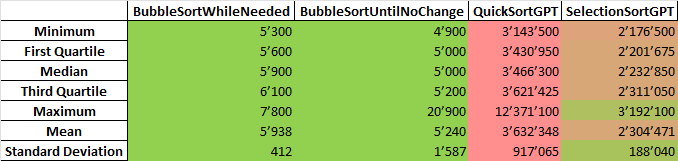
\includegraphics[width=0.75\linewidth]{char1000sort-stat.png}
        \caption{Statistics for char[1000] sorted}
        \label{fig:char1000sort-stat}
    \end{figure}
    \begin{figure}[!h]
        \centering
        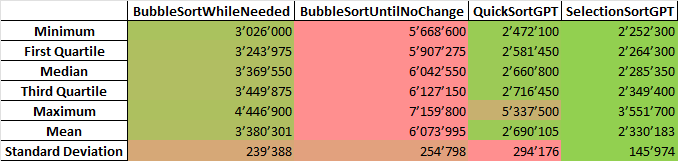
\includegraphics[width=0.75\linewidth]{char1000rev-stat.png}
        \caption{Statistics for char[1000] reverse}
        \label{fig:char1000rev-stat}
    \end{figure}
    \begin{figure}[!h]
        \centering
        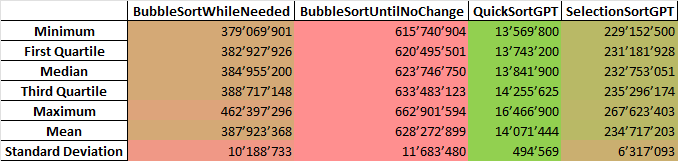
\includegraphics[width=0.75\linewidth]{char10000rand-stat.png}
        \caption{Statistics for char[10000] random filled}
        \label{fig:char10000rand-stat}
    \end{figure}
    \begin{figure}[!h]
        \centering
        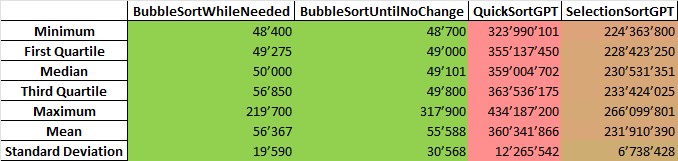
\includegraphics[width=0.75\linewidth]{char10000sort-stat.png}
        \caption{Statistics for char[10000] sorted}
        \label{fig:char10000sort-stat}
    \end{figure}
    \begin{figure}[!h]
        \centering
        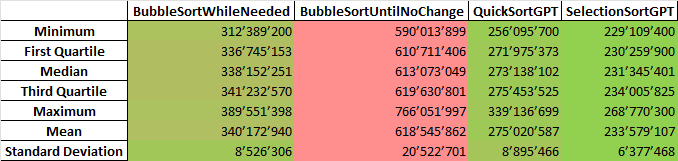
\includegraphics[width=0.75\linewidth]{char10000rev-stat.png}
        \caption{Statistics for char[10000] reverse}
        \label{fig:char10000rev-stat}
    \end{figure}
    \begin{figure}[!h]
        \centering
        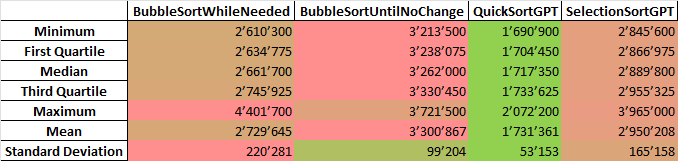
\includegraphics[width=0.75\linewidth]{bool1000rand-stat.png}
        \caption{Statistics for bool[1000] random filled}
        \label{fig:bool1000rand-stat}
    \end{figure}
    \begin{figure}[!h]
        \centering
        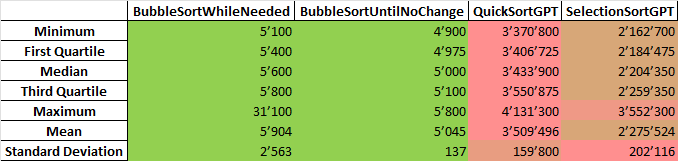
\includegraphics[width=0.75\linewidth]{bool1000sort-stat.png}
        \caption{Statistics for bool[1000] sorted}
        \label{fig:bool1000sort-stat}
    \end{figure}
    \begin{figure}[!h]
        \centering
        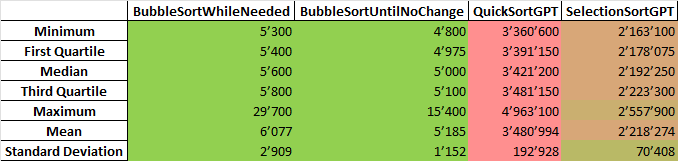
\includegraphics[width=0.75\linewidth]{bool1000rev-stat.png}
        \caption{Statistics for bool[1000] reverse}
        \label{fig:bool1000rev-stat}
    \end{figure}
    \begin{figure}[!h]
        \centering
        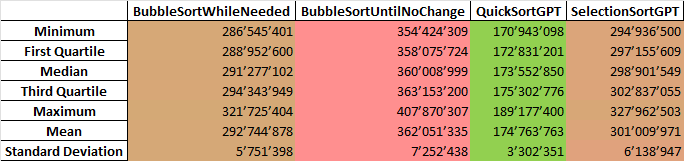
\includegraphics[width=0.75\linewidth]{bool10000rand-stat.png}
        \caption{Statistics for bool[10000] random filled}
        \label{fig:bool10000rand-stat}
    \end{figure}
    \begin{figure}[!h]
        \centering
        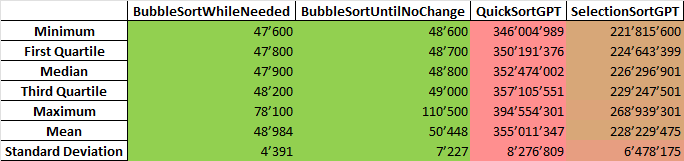
\includegraphics[width=0.75\linewidth]{bool10000sort-stat.png}
        \caption{Statistics for bool[10000] sorted}
        \label{fig:bool10000sort-stat}
    \end{figure}
    \begin{figure}[!h]
        \centering
        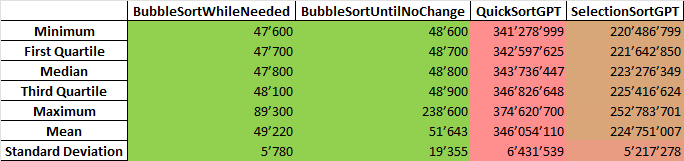
\includegraphics[width=0.75\linewidth]{bool10000rev-stat.png}
        \caption{Statistics for bool[10000] reverse}
        \label{fig:bool10000rev-stat}
    \end{figure}
    
\clearpage
\newpage

\section{Discussion}
    \subsection{Compare Hypothesis to Results}
    Analyzing the results obtained, we find that the performance of the graphs representing the sorting time of the various algorithms is very similar between the tests done on the 1,000-elements and 10,000-elements arrays. So all algorithms suffer from the same “scalability” based on the size of the data to be sorted. This allows us to make a more general analysis since in this respect the algorithms are nearly equivalent.\\
    
    Our initial hypothesis was formulated considering the average use case of the sorting algorithms, so with a shuffled array. \\

    That said, we had not considered edge cases where one might find oneself having to order arrays that are already sorted, or reverse-sorted.
    
    So analyzing these edge cases as well, we can see that rightly so when dealing with already sorted arrays, the BubbleSortWhileNeeded and BubbleSortUntilNoChange algorithms perform excellently when compared to QuickSortGPT or SelectionSortGPT. But this was to be expected given the very nature of the algorithms, which, precisely, if the array turns out to be already sorted, need only iterate over it without performing any extra operations. However, this case cannot represent a “relevant” example since we imagine there would be no need to sort an already sorted array, and therefore it would not make sense to use the implemented library.
    
    In the case of the revert-sorted array, we lose this “advantage” of the two BubbleSorts over QuickSortGPT and SelectionSortGPT by finding, precisely for the BubbleSorts, equal or worse performance than in the average case (random filled array). \\ 
    However, we find that in this case, the best performing algorithm would turn out to be SelectionSortGPT. Looking at the values, however, we find that SelectionSortGPT tends to (with the same type of data) have performance that is about 15\% better than that of QuickSortGPT; in contrary, with randomly filled arrays, QuickSortGPT has performance that is around 90\% better than SelectionSortGPT.\\

    Thus, considering the average use case, that is, the one represented by randomly filled arrays, we find that the best performing algorithm is QuickSortGPT.
    
    This confirms our initial hypothesis that, in average case, the complexity of QuickSort, i.e., $O(n*logn)$, leads it to be the best performing algorithm compared to the proposed competitors.
    
%         This analysis examines the performance of several sorting algorithms (BubbleSortWhileNeeded, BubbleSortUntilNoChange, QuickSort, and SelectionSort) across datasets of different sizes (1000 and 10000 elements) and orderings (random, sorted, and reverse sorted). The key metrics considered include minimum, first quartile, median, third quartile, maximum, mean, and standard deviation of runtimes.

% \paragraph{Detailed Observations}

% \subparagraph{1. BubbleSortWhileNeeded and BubbleSortUntilNoChange}
% \begin{itemize}
%     \item \textbf{Performance with array size}: Both BubbleSort variants show significantly higher values in terms of mean and maximum runtime for the 10000 element arrays compared to the 1000 element arrays, as expected with increased data size. For example, the mean runtime of \texttt{BubbleSortWhileNeeded} with \texttt{10000\_random} is much higher than with \texttt{1000\_random}.
%     \item \textbf{Effect of ordering}:
%     \begin{itemize}
%         \item Sorted arrays yield the lowest runtime across all sorting algorithms, with \texttt{BubbleSortWhileNeeded} and \texttt{BubbleSortUntilNoChange} benefiting notably when the data is already sorted. Their runtimes are substantially lower with sorted arrays than with random or reverse-sorted arrays.
%         \item Reverse-sorted arrays generally have higher runtime compared to sorted ones, but they still benefit \texttt{BubbleSortUntilNoChange} since the numr of required comparisons decreases over time.
%     \end{itemize}
% \end{itemize}

% \subparagraph{2. QuickSort}
% \begin{itemize}
%     \item \textbf{Consistency across orderings}: QuickSort's runtimes show less variation across sorted, reverse-sorted, and random arrays compared to BubbleSort, although random order arrays sometimes have slightly higher runtimes due to partitioning.
%     \item \textbf{Scalability with size}: The increase in mean and maximum runtime from 1000 to 10000 elements is present but much less dramatic than in BubbleSort, indicating QuickSort's superior efficiency and scalability with large datasets.
% \end{itemize}

% \subparagraph{3. SelectionSort}
% \begin{itemize}
%     \item \textbf{Performance trend}: SelectionSort exhibits a higher runtime in random and reverse-sorted arrays compared to sorted arrays, though not as high as the BubbleSort algorithms for similar data sizes and orderings.
%     \item \textbf{Scalability limitations}: SelectionSort’s performance with larger datasets (10000 elements) reveals an exponential increase in runtime, similar to BubbleSort, due to its $O(n^2)$ complexity. This makes it much slower for larger datasets compared to QuickSort.
% \end{itemize}

% \subparagraph{4. Impact of Sorted and Reverse-Sorted Inputs}
% \begin{itemize}
%     \item \textbf{Sorted data}: All algorithms, especially BubbleSort and SelectionSort, benefit considerably from sorted inputs, with lower values across all statistics.
%     \item \textbf{Reverse-sorted data}: Reverse sorting tends to increase the workload for BubbleSort variants, although not as dramatically as for completely random inputs. QuickSort and SelectionSort are affected but maintain a level of consistency.
% \end{itemize}

% \subparagraph{5. General Observations}
% \begin{itemize}
%     \item \textbf{Efficiency across algorithms}: QuickSort shows the lowest runtimes and best scalability overall, supporting its reputation as a highly efficient sorting algorithm, particularly for larger datasets.
%     \item \textbf{Inefficiency in BubbleSort}: The BubbleSort variants, especially \texttt{BubbleSortUntilNoChange}, show high variability in runtime depending on the input ordering and data size, highlighting their inefficiency for larger datasets.
%     \item \textbf{Order of magnitude in differences}: Runtime increases with data size are exponential in BubbleSort and SelectionSort due to $O(n^2)$ complexity, contrasting with QuickSort's more manageable increase.
% \end{itemize}

% \paragraph{Conclusion}
% In summary, QuickSort consistently outperforms BubbleSort and SelectionSort in both efficiency and scalability, especially with larger datasets. This aligns with theoretical expectations and demonstrates the performance limitations of BubbleSort and SelectionSort, particularly in handling large or unsorted data.
    \subsection{Limitations and Threats to Validity}
    Some of the factors that we can consider as limitations in terms of ensuring absolute validity of our experiment may be the following:
    \begin{itemize}
        \item \textbf{Hardware constrains:} We conducted the tests on a single machine; thus, our results are dependent on the hardware's performance, and we lack a comparison with other machines with different hardware configurations. It might have been interesting to perform the same tests on sample machines similar to those on which Bubble Inc. expects its library to be used, in order to ensure that the obtained results are consistent.
        \item \textbf{Background processes:} Even by trying to limit this issue by restarting the machine before each measurement, the number of active background processes and applications can still influence the performance of various algorithms to some extent, potentially leading to different results.
        \item \textbf{Performance measurement:} Using Java's \texttt{System.nanoTime()} function to measure sorting time may result in inaccuracies due to the machine's clock and interference from certain background processes. In any case, the potential variations would be minimal so we do not think this would be a real limitation (but it is still a present factor, so we wanted to mention it).
        \item \textbf{Scope of tested cases:} Although we attempted to test many variations of arrays in terms of size and data type, these variations are limited. For a more precise and accurate analysis, we could have tested additional variations in terms of array size and data type. We could also have used different filling patterns for the arrays, mixing portions that are already sorted, reversed, or random.
        \item \textbf{Reliability of measurements:} To ensure a good level of reliability, we performed 100 repetitions of each sorting combination. However, this number of repetitions may still be vulnerable to external biases (such as background processes) and thus might not be sufficiently high. The greater the number of repetitions, the higher the reliability of the average value obtained. \\ We decided to keep this value at 100 repetitions because by analyzing the trends in the graphs for the timing of the various algorithms (as can be seen in chapter \textit{5.3 Additional Figures}), they all appear to be stable and more or less constant from the very first iterations (due to the fact that we performed the warm-up). So 100 seemed to us a good compromise to ensure reliability of the results without repeating measurements that would follow the same trend as those already performed.
    \end{itemize}

    \subsection{Conclusions}
    In conclusion, we can confirm that our initial hypothesis, according to which the QuickSortGPT algorithm would perform best on random arrays (thanks to its Average Time Complexity of \texttt{O(n*logn)}), has been proven correct.\\
    
    We also noticed that both variants of BubbleSort perform very well on pre-ordered arrays but poorly on unordered datasets (both random and reversed). However, having pre-ordered datasets is quite an unrealistic scenario, which makes both versions unsuitable for general real-world applications.
    
    Similarly, SelectionSortGPT has a scenario in which it performs the best among all the proposed algorithms, specifically when the dataset is reversed. But again, this is a very unlikely scenario in the real world, making it unsuitable.\\
    
    Considering the goal of the research, with the aim of implementing this sorting algorithm within a library for Bubble Inc as a "utility tool," and given that we have no control over the datasets it will be used with (thus relying on randomized datasets), we suggest the implementation of the QuickSortGPT algorithm.

\newpage

\section{Appendix}\label{chap:appendix}
    \subsection{Materials}
    The documents we used as reference material for this research are the slides from the "Experimentation and Evaluation" course.

    \subsection{Reproduction Package}
    All the resources we used, such as Java files, CSV files from which we generated the charts, Excel files used for chart representation, etc., are all available in the following GitHub repository: \\
    \url{https://github.com/ghi-la/Experimentation-Evaluation}
    
    \subsection{Additional Figures}
    \begin{figure}[!h]
        \centering
        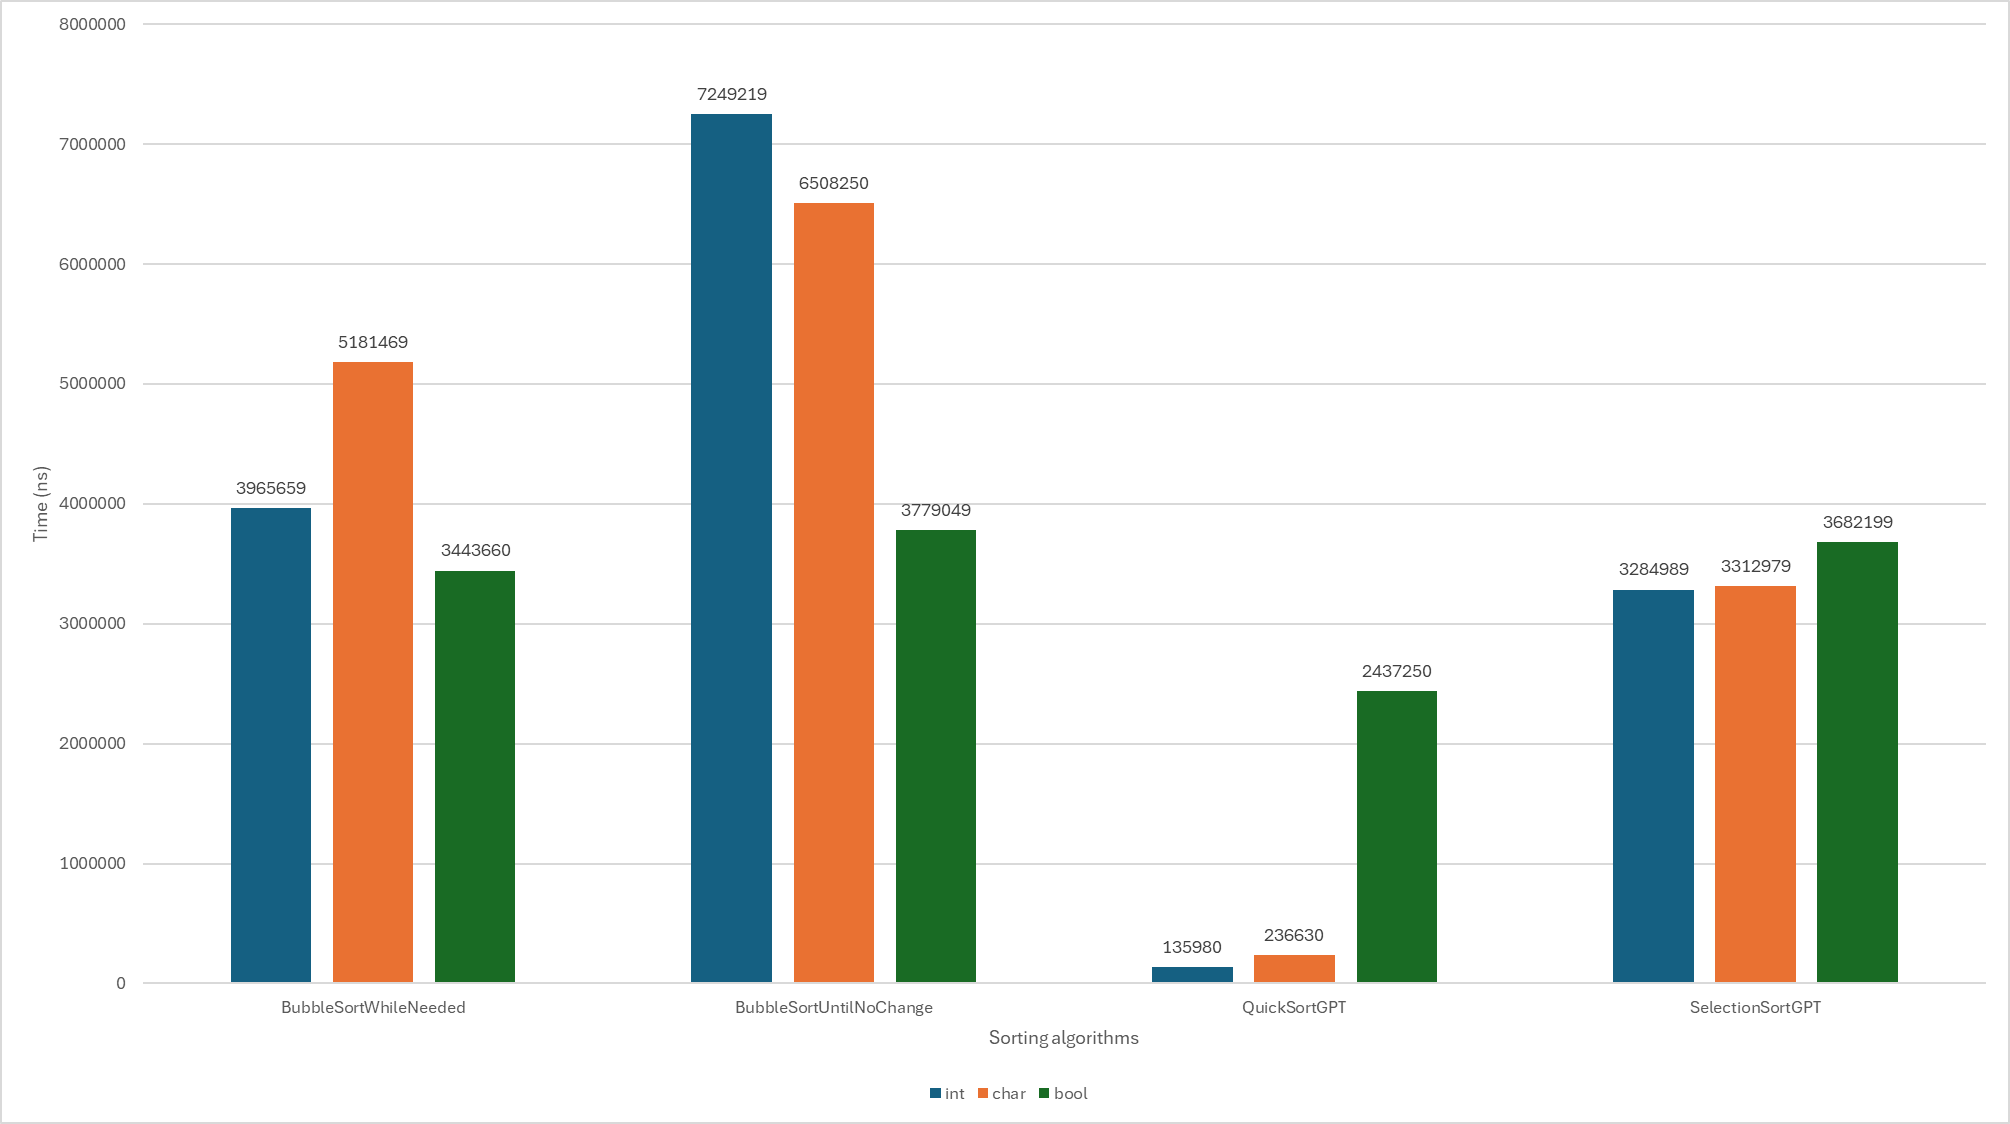
\includegraphics[width=0.75\linewidth]{warmup_avg_1000.png}
        \caption{Statistics for the warm up average of a randomly filled array of size 1000}
        \label{fig:warmup_avg_1000_random}
    \end{figure}

    %int
    
    \begin{figure}[!h]
        \centering
        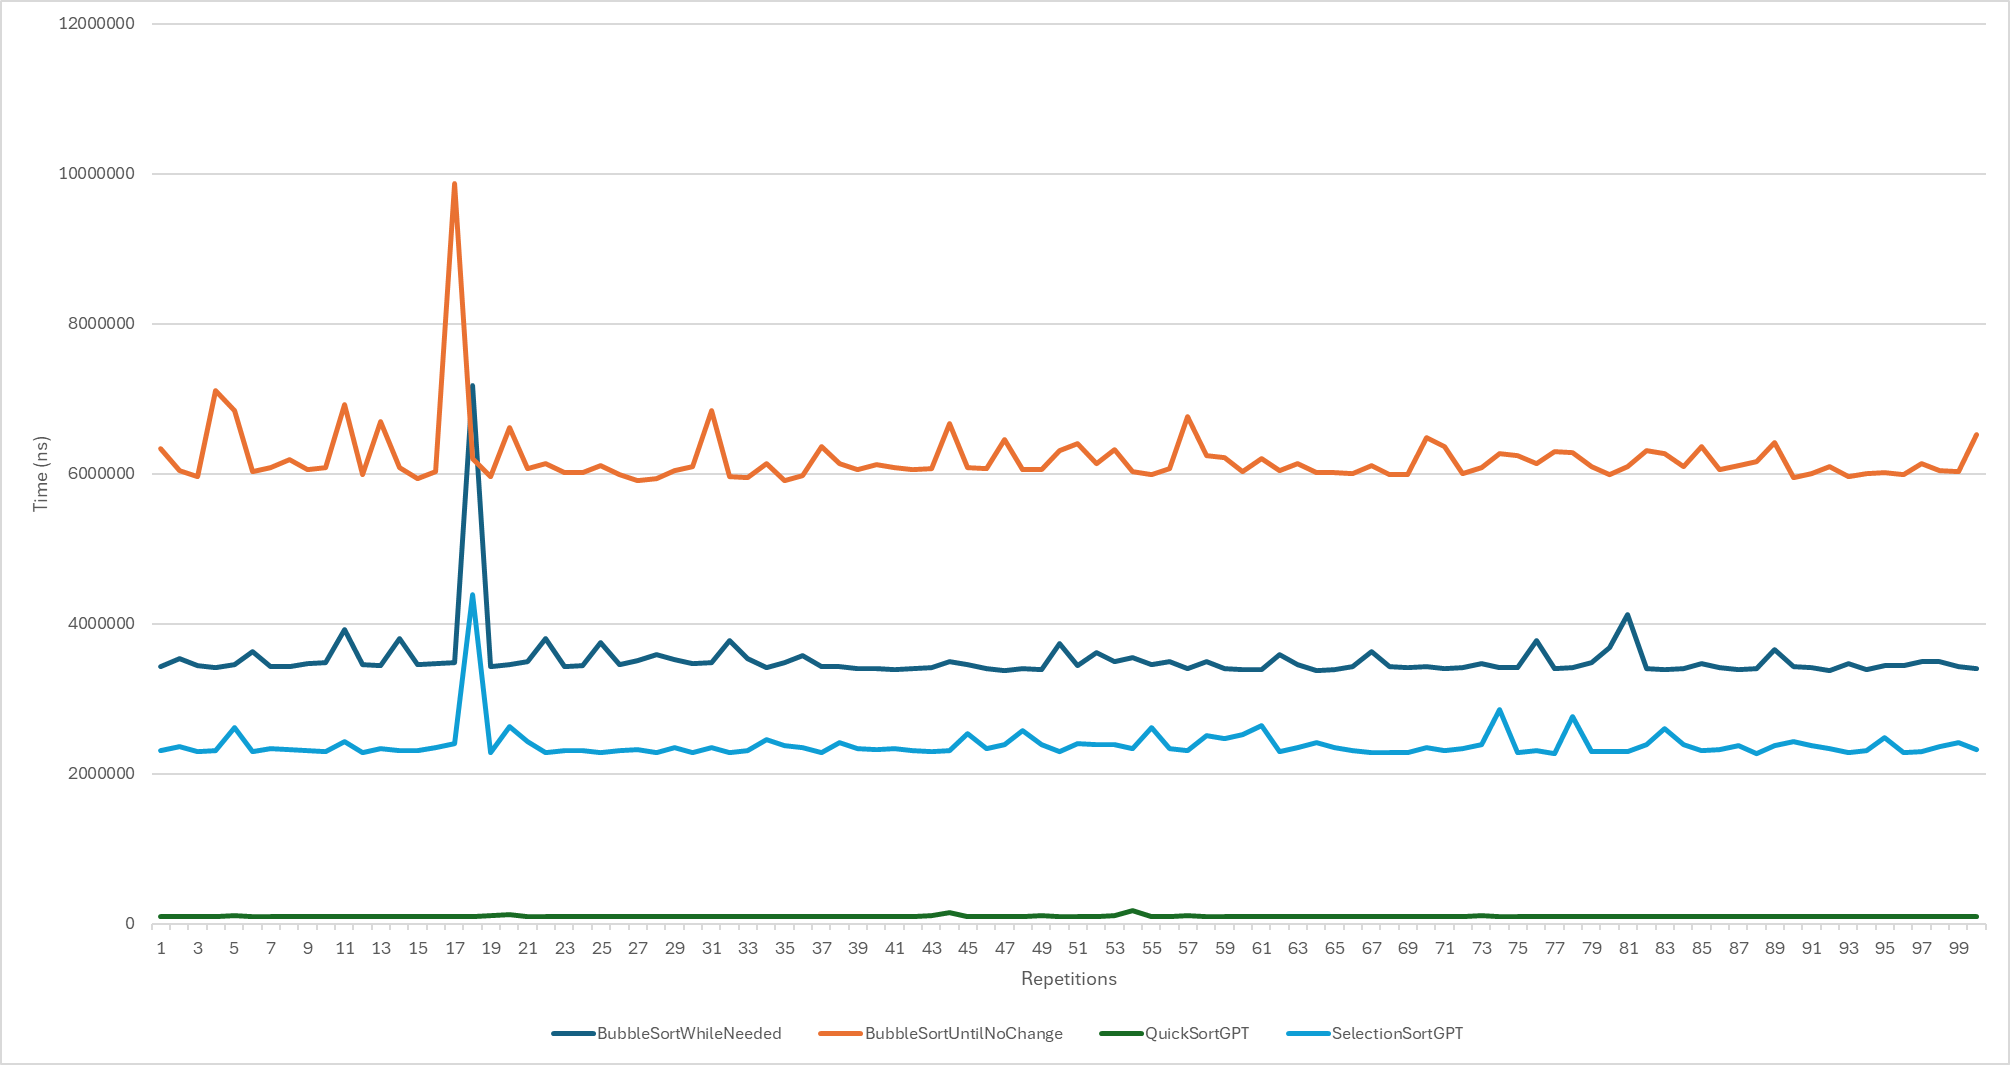
\includegraphics[width=0.7\linewidth]{int_1000_random.png}
        \caption{Results of sorting a randomly filled array of size 1000 made from int}
        \label{fig:int_1000_random}
    \end{figure}
    
    \begin{figure}[!h]
        \centering
        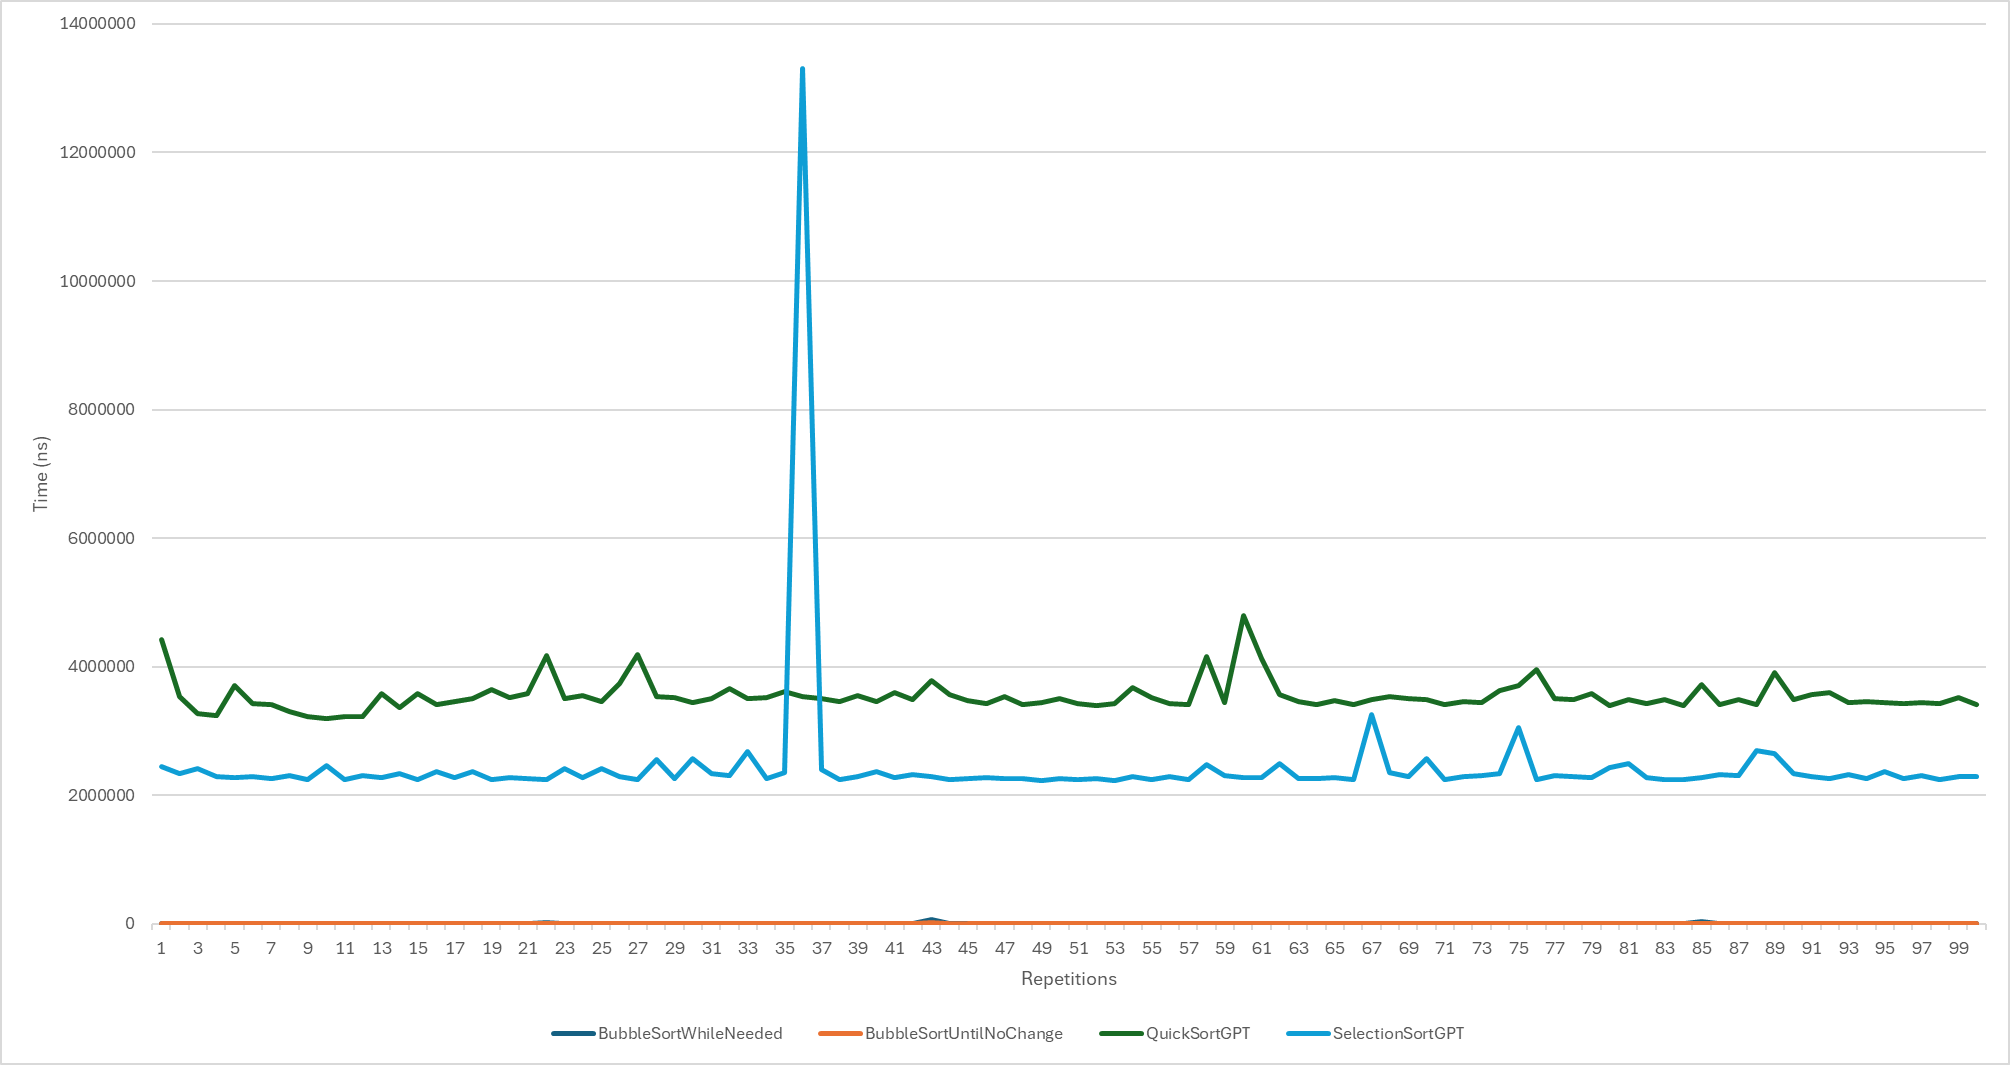
\includegraphics[width=0.7\linewidth]{int_1000_sorted.png}
        \caption{Results of sorting a sorted array of size 1000 made from int}
        \label{fig:int_1000_sorted}
    \end{figure}
    
    \begin{figure}[!h]
        \centering
        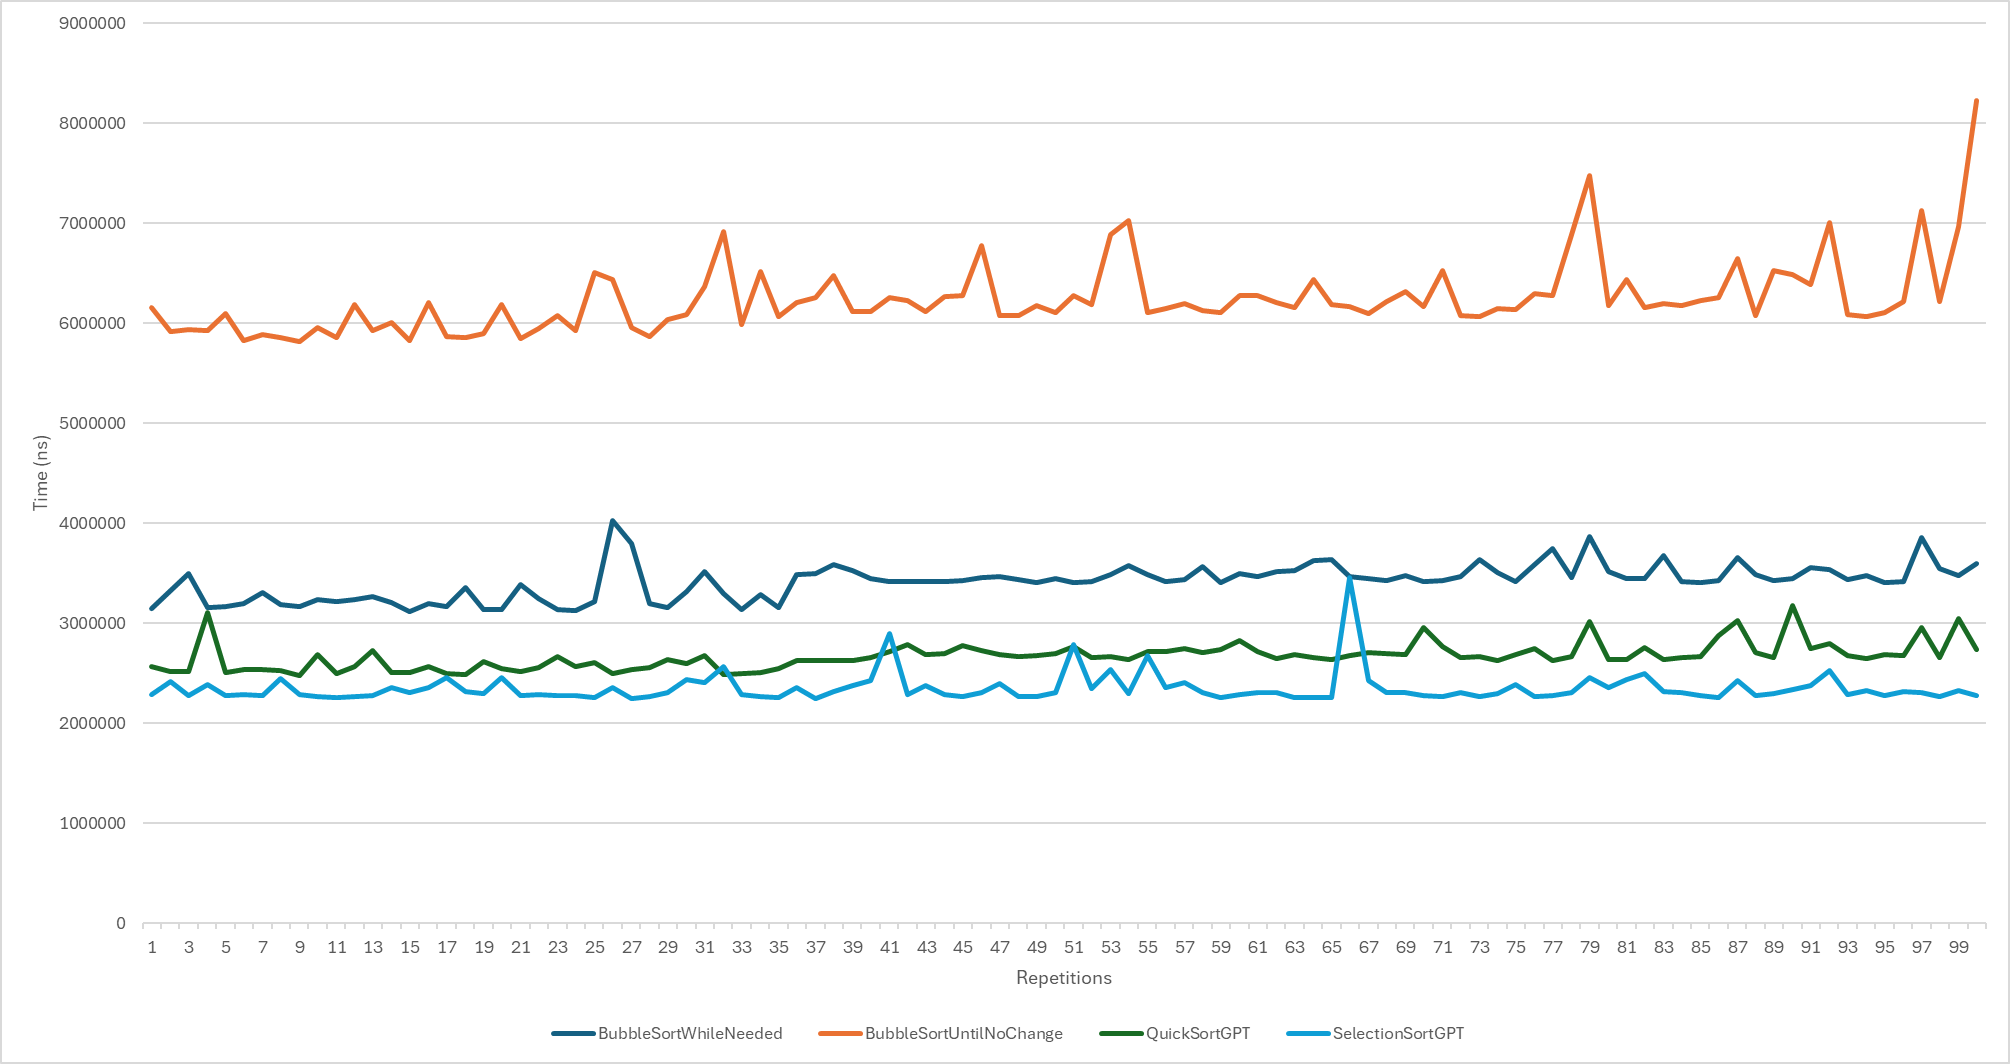
\includegraphics[width=0.7\linewidth]{int_1000_reverse_sorted.png}
        \caption{Results of sorting a reverse sorted array of size 1000 made from int}
        \label{fig:int_1000_reverse_sorted}
    \end{figure}
    
    \begin{figure}[!h]
        \centering
        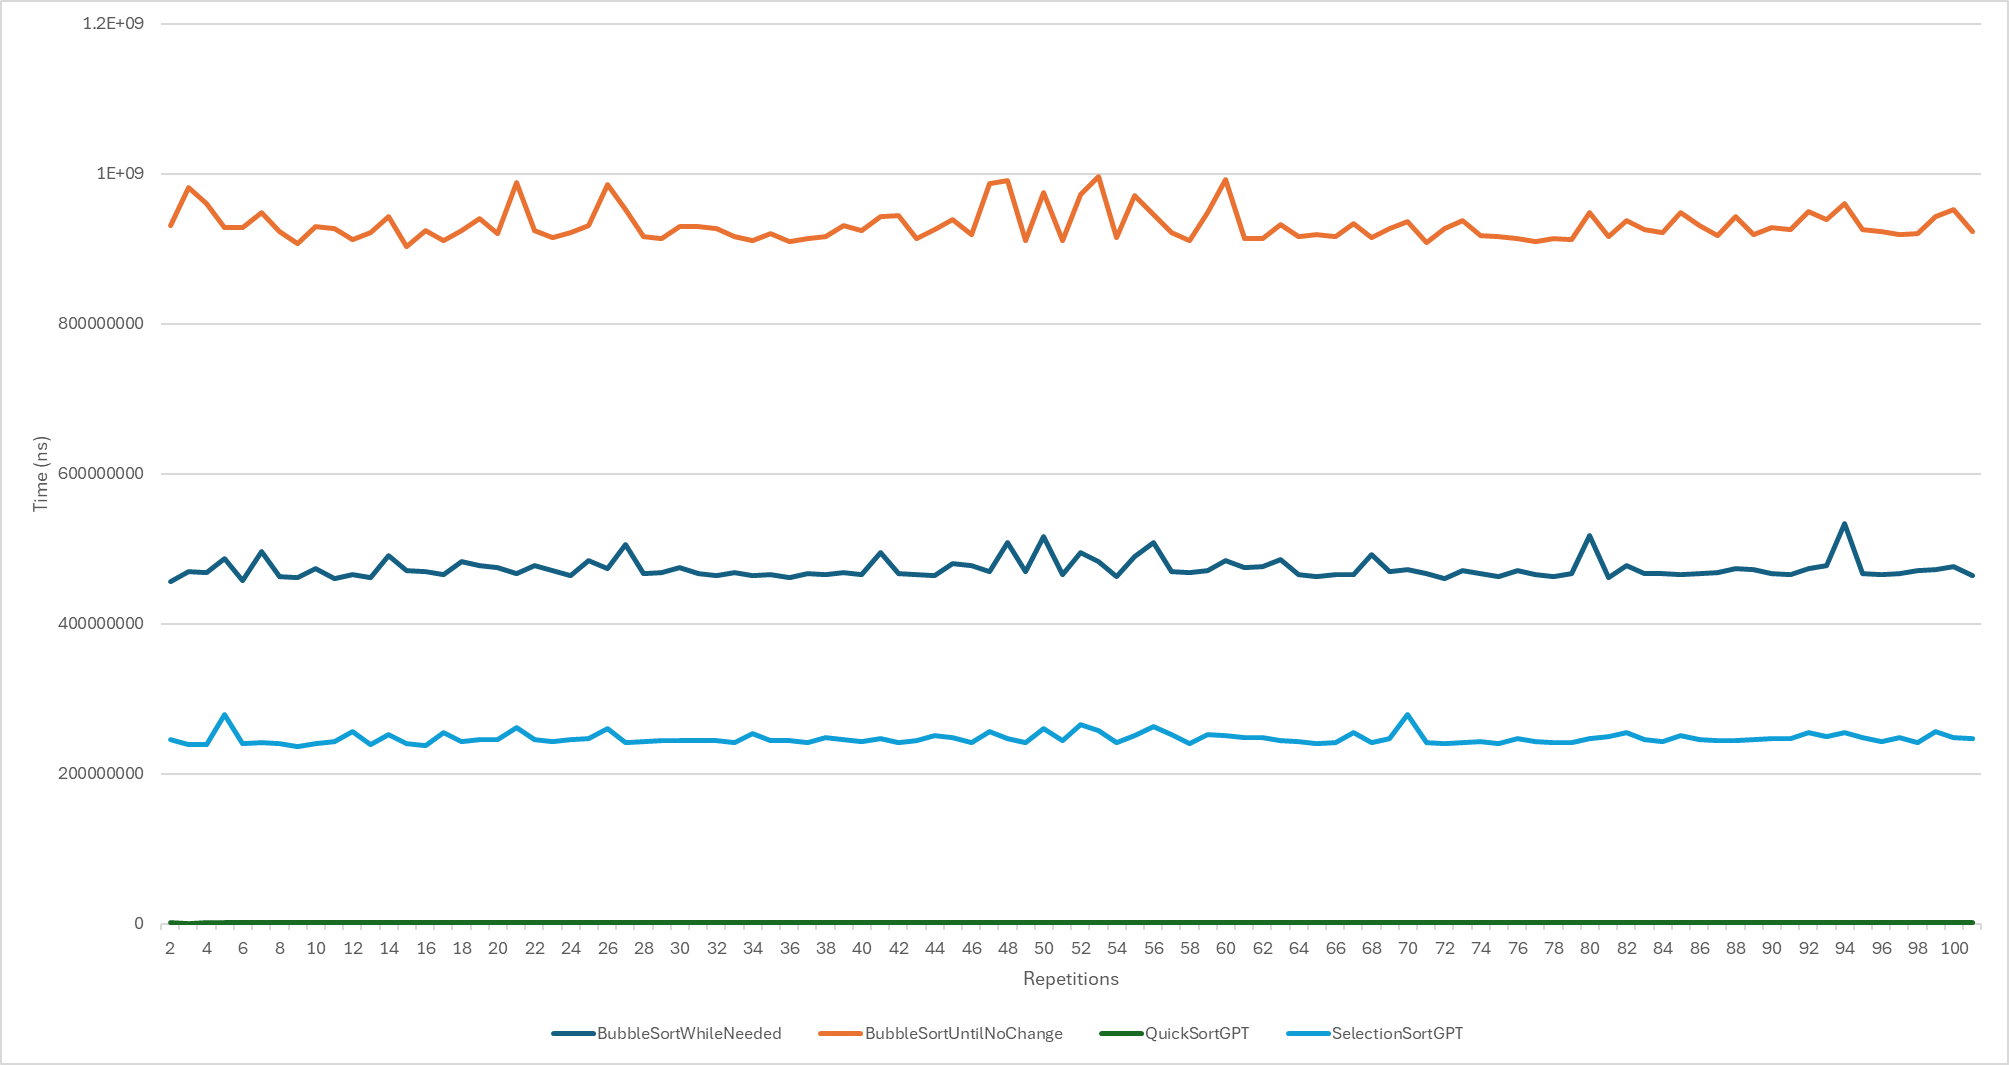
\includegraphics[width=0.7\linewidth]{int_10000_random.png}
        \caption{Results of sorting a randomly filled array of size 10000 made from int}
        \label{fig:int_10000_random}
    \end{figure}
    
    \begin{figure}[!h]
        \centering
        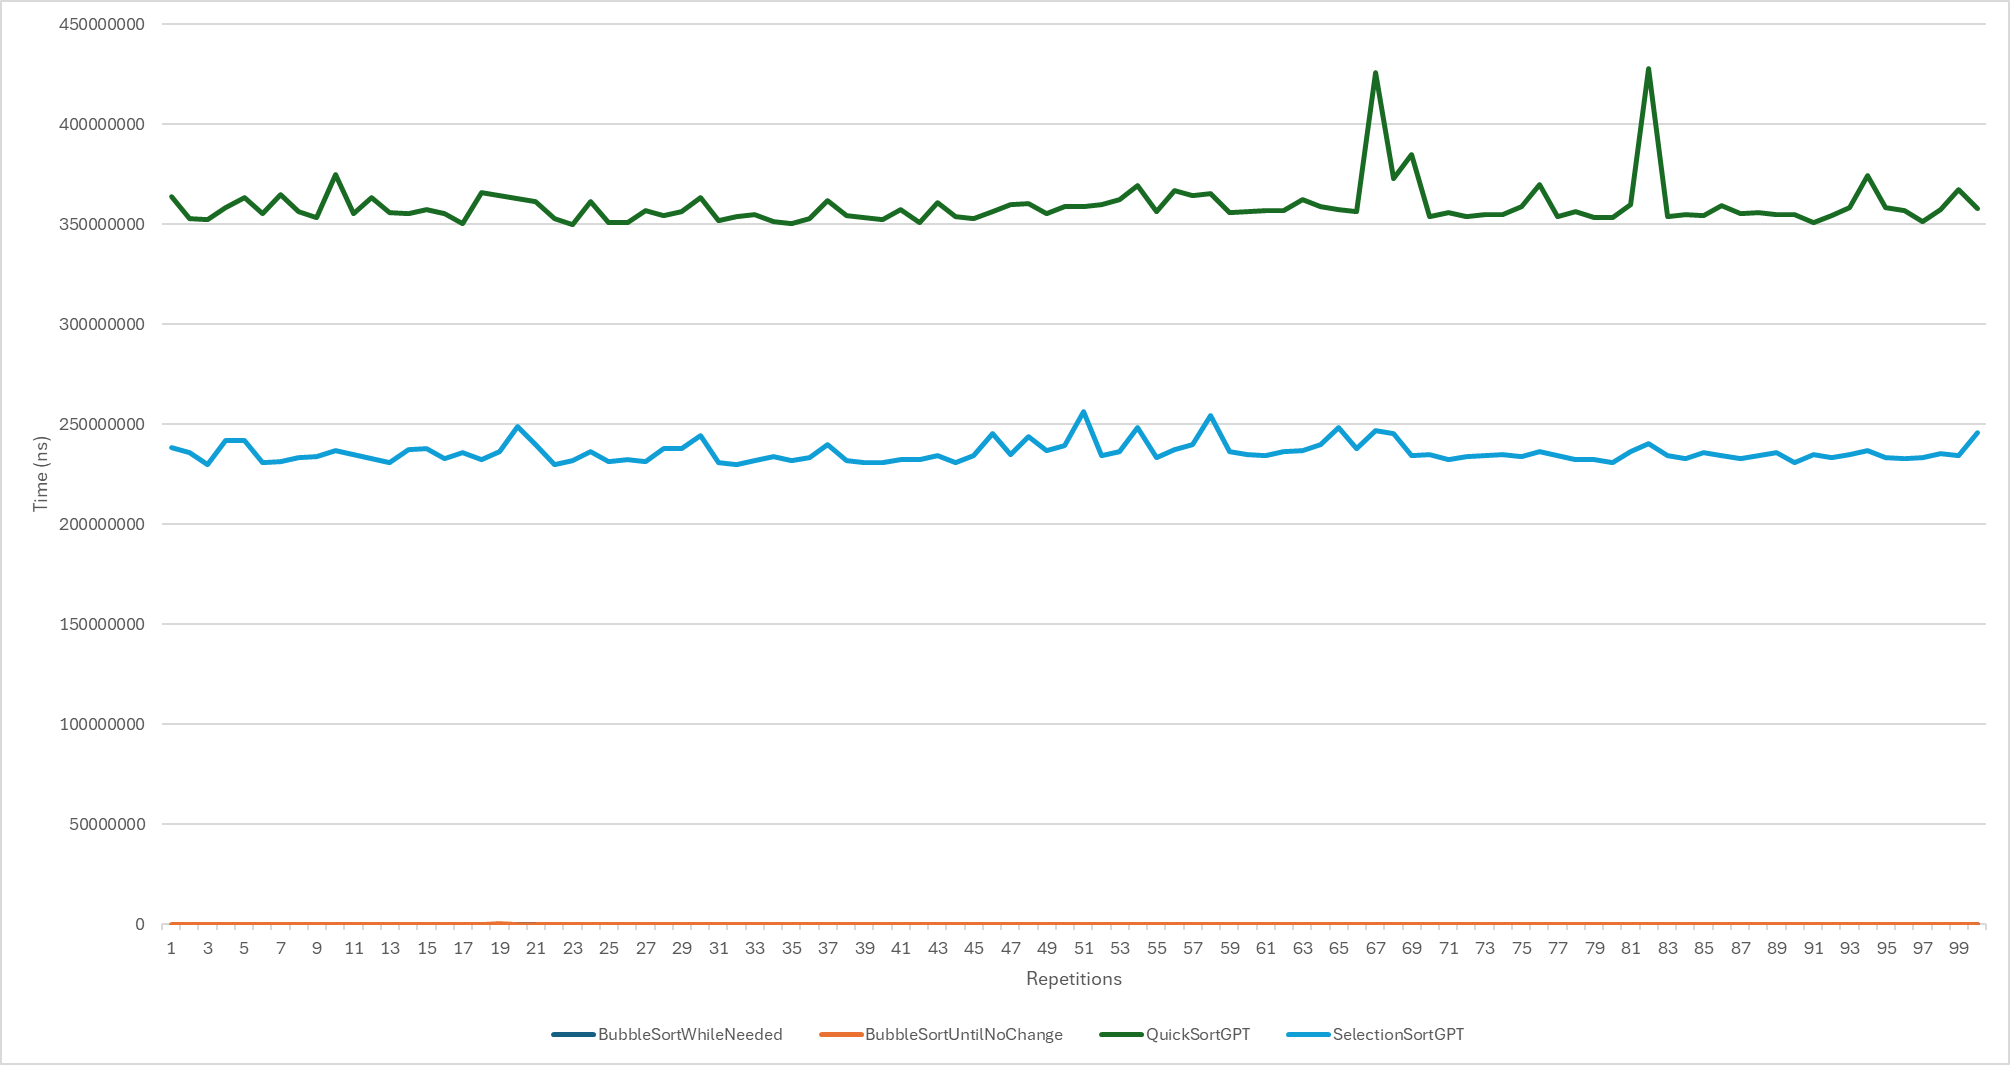
\includegraphics[width=0.7\linewidth]{int_10000_sorted.png}
        \caption{Results of sorting a sorted array of size 10000 made from int}
        \label{fig:int_10000_sorted}
    \end{figure}
    
    \begin{figure}[!h]
        \centering
        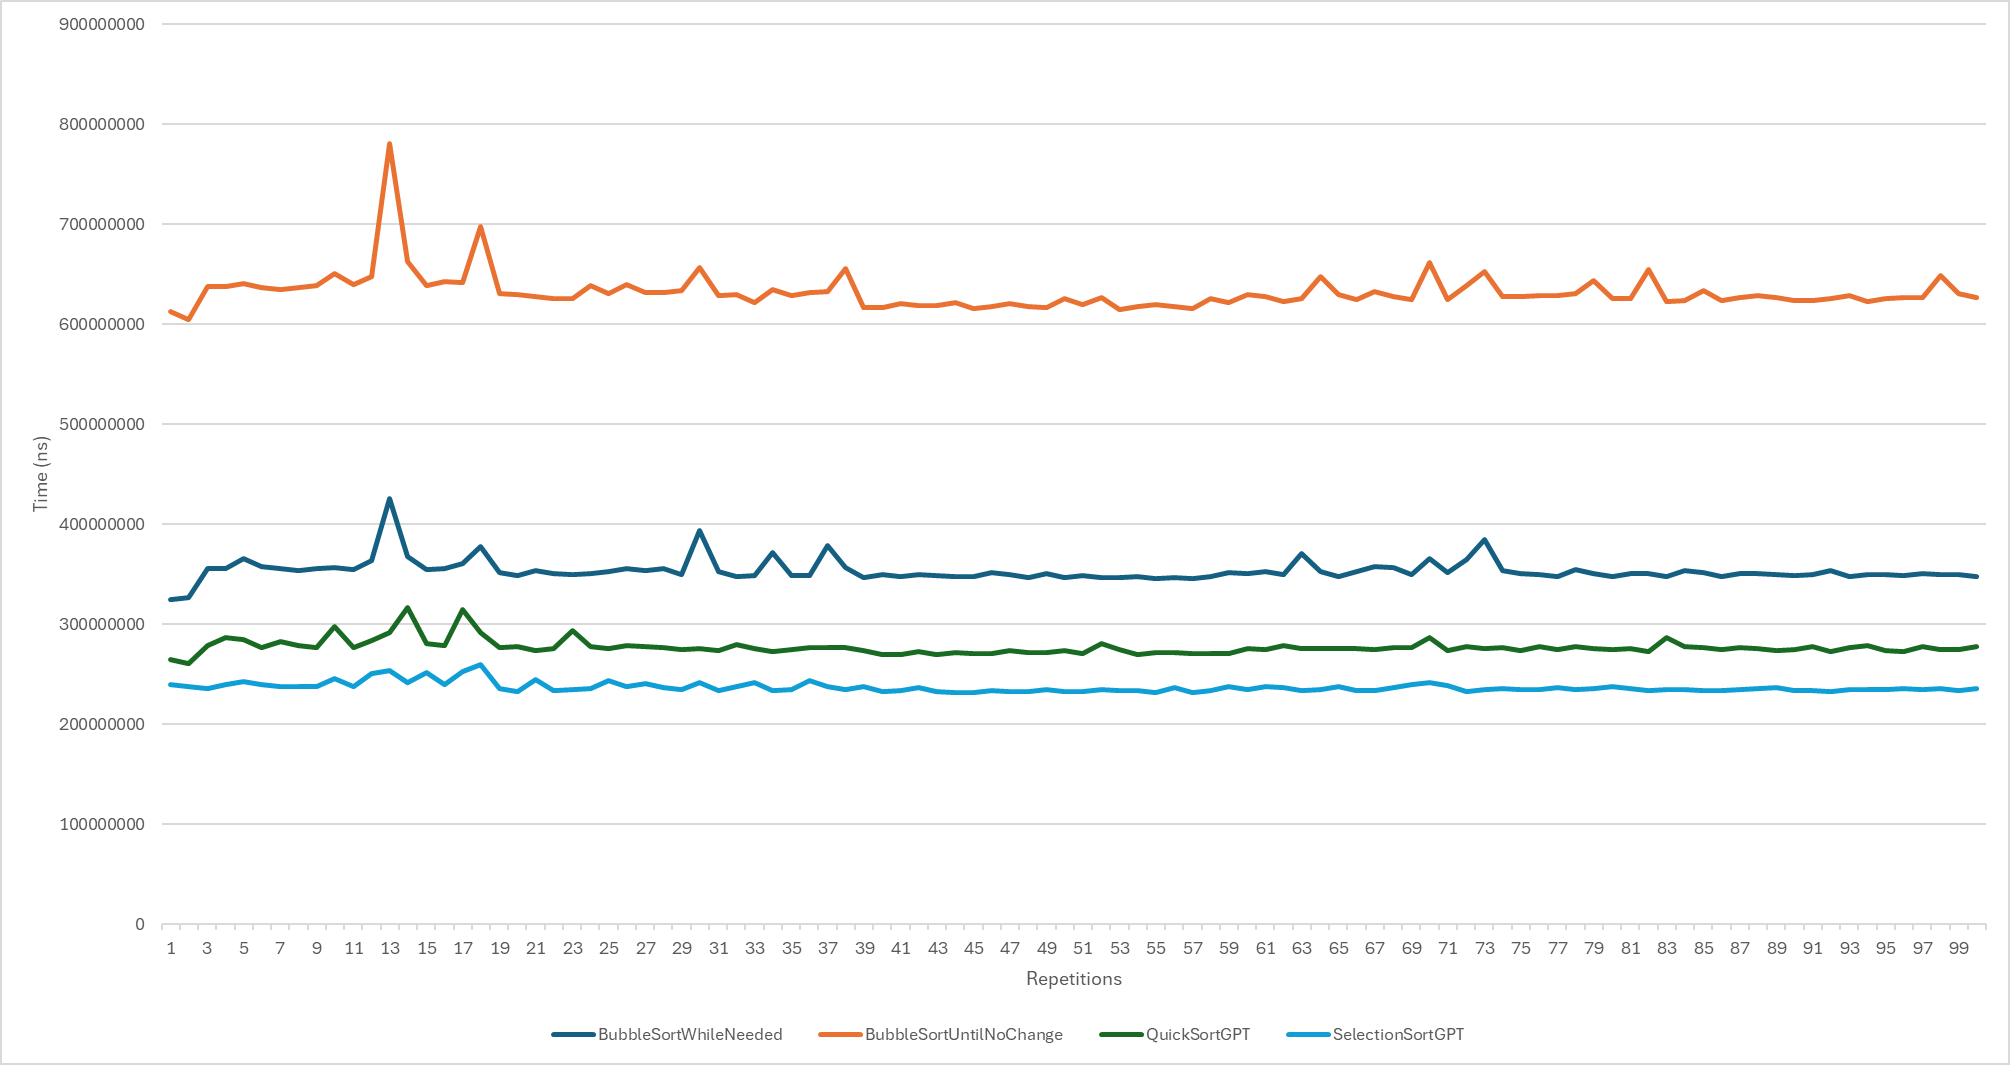
\includegraphics[width=0.7\linewidth]{int_10000_reverse_sorted.png}
        \caption{Results of sorting a reverse sorted array of size 10000 made from int}
        \label{fig:int_10000_reverse_sorted}
    \end{figure}

    %char

    \begin{figure}[!h]
        \centering
        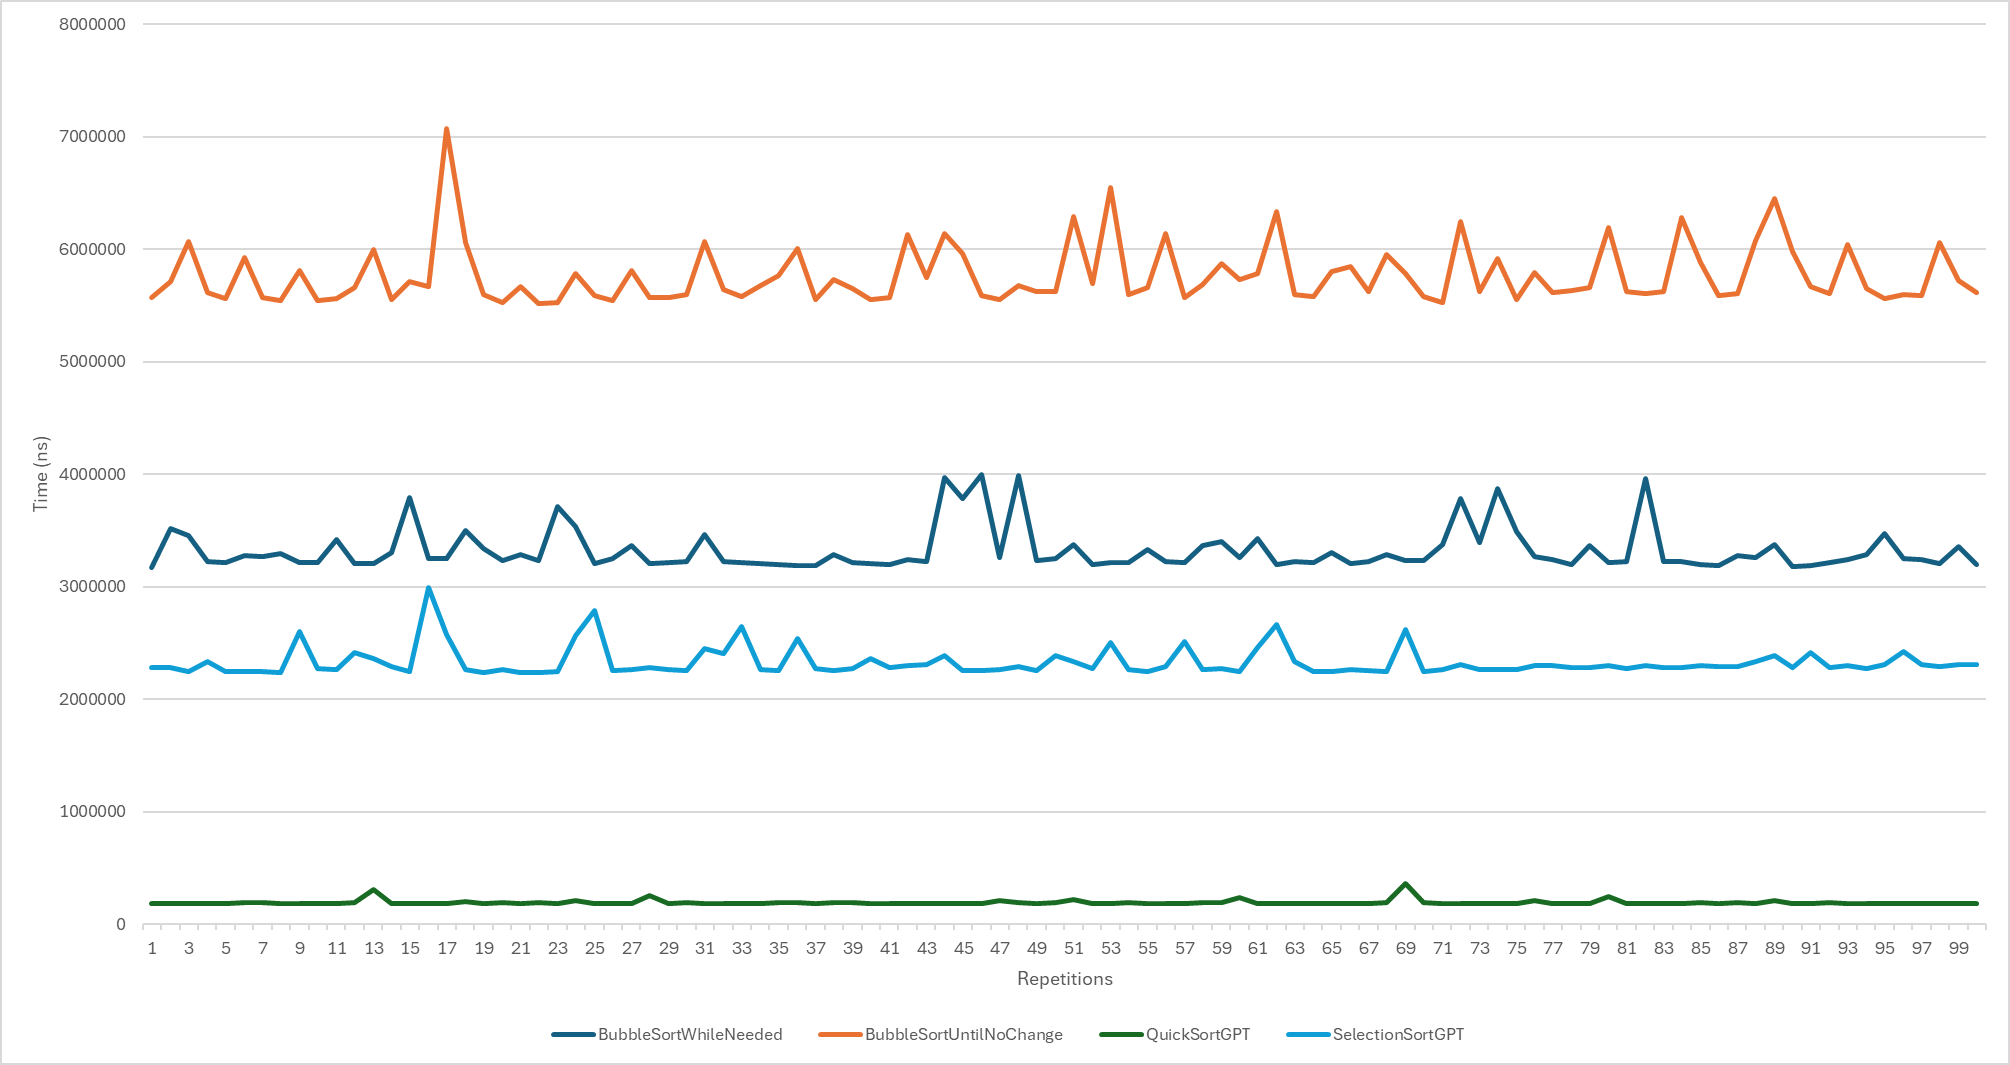
\includegraphics[width=0.7\linewidth]{char_1000_random.png}
        \caption{Results of sorting a randomly filled array of size 1000 made from char}
        \label{fig:char_1000_random}
    \end{figure}
    
    \begin{figure}[!h]
        \centering
        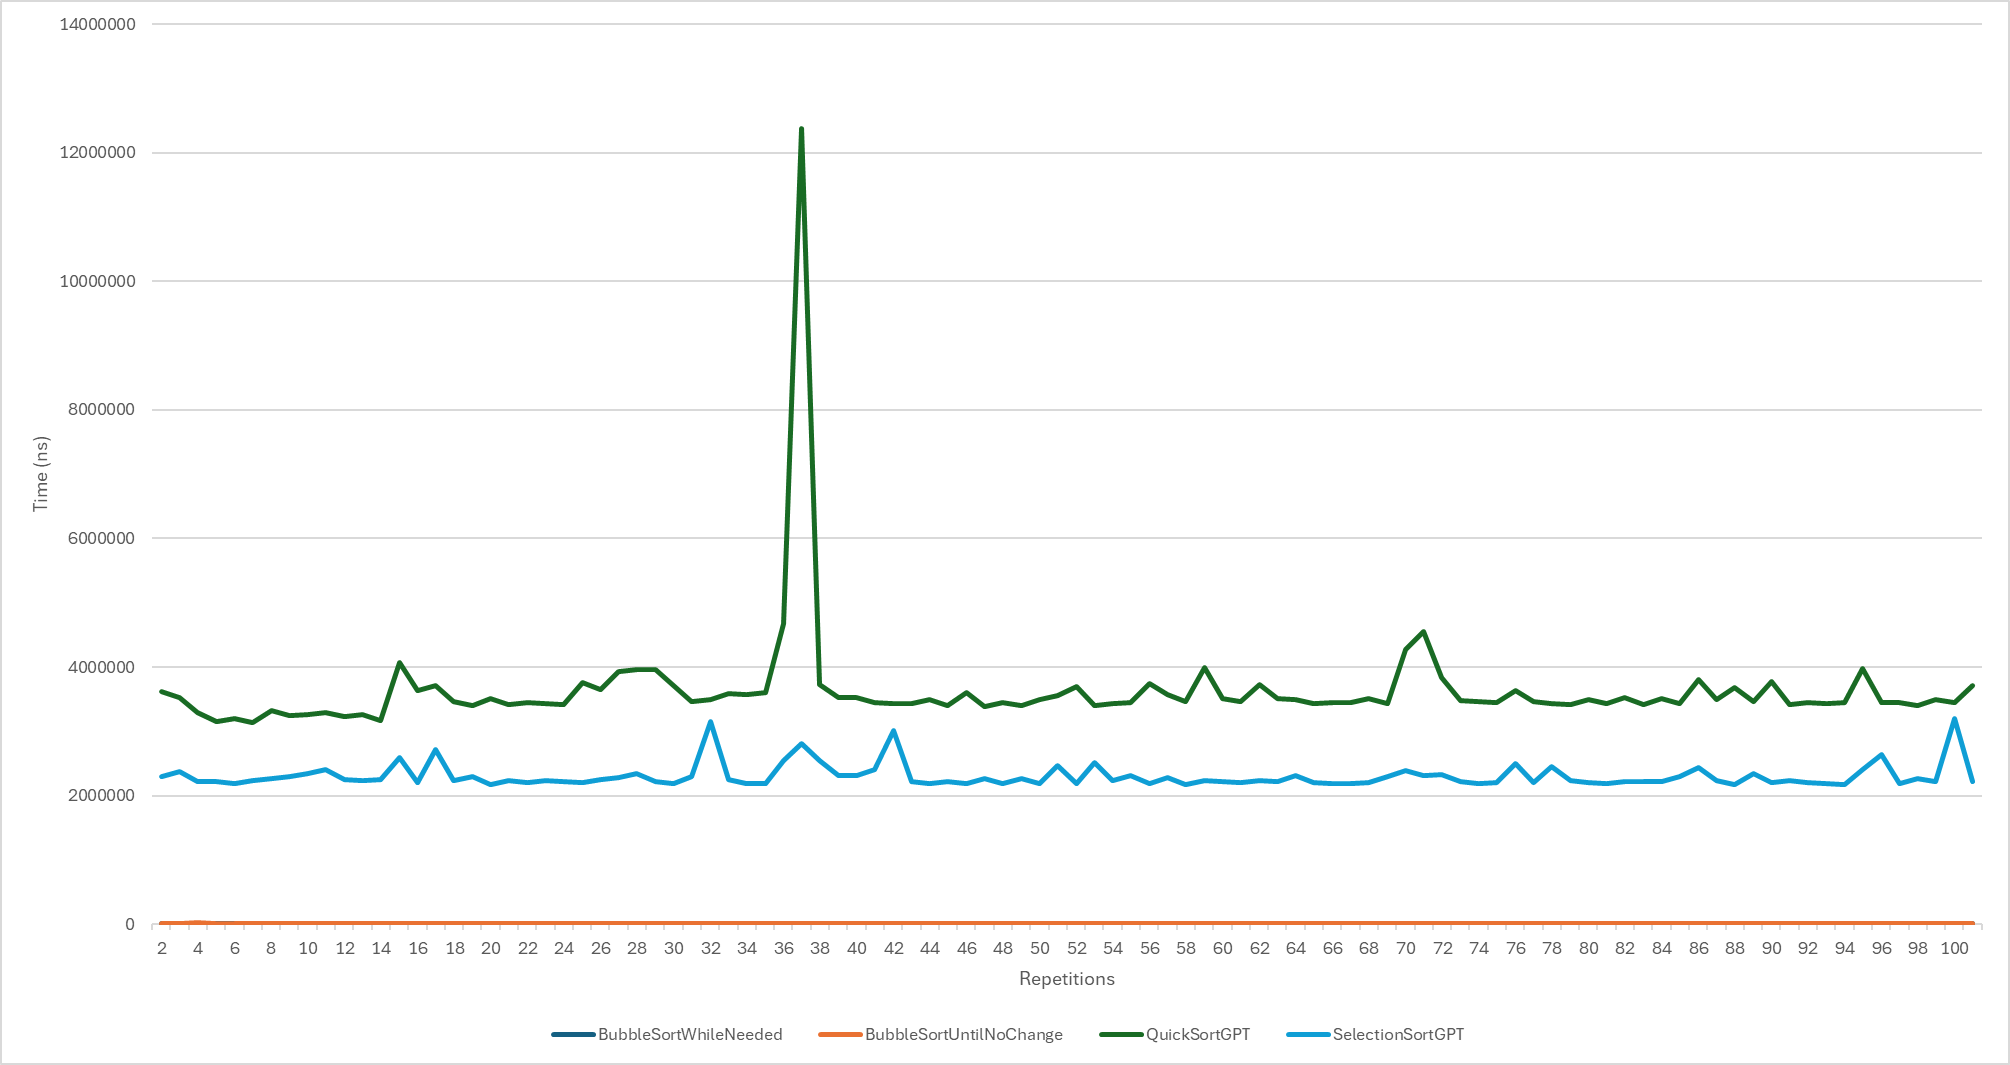
\includegraphics[width=0.7\linewidth]{char_1000_sorted.png}
        \caption{Results of sorting a sorted array of size 1000 made from char}
        \label{fig:char_1000_sorted}
    \end{figure}
    
    \begin{figure}[!h]
        \centering
        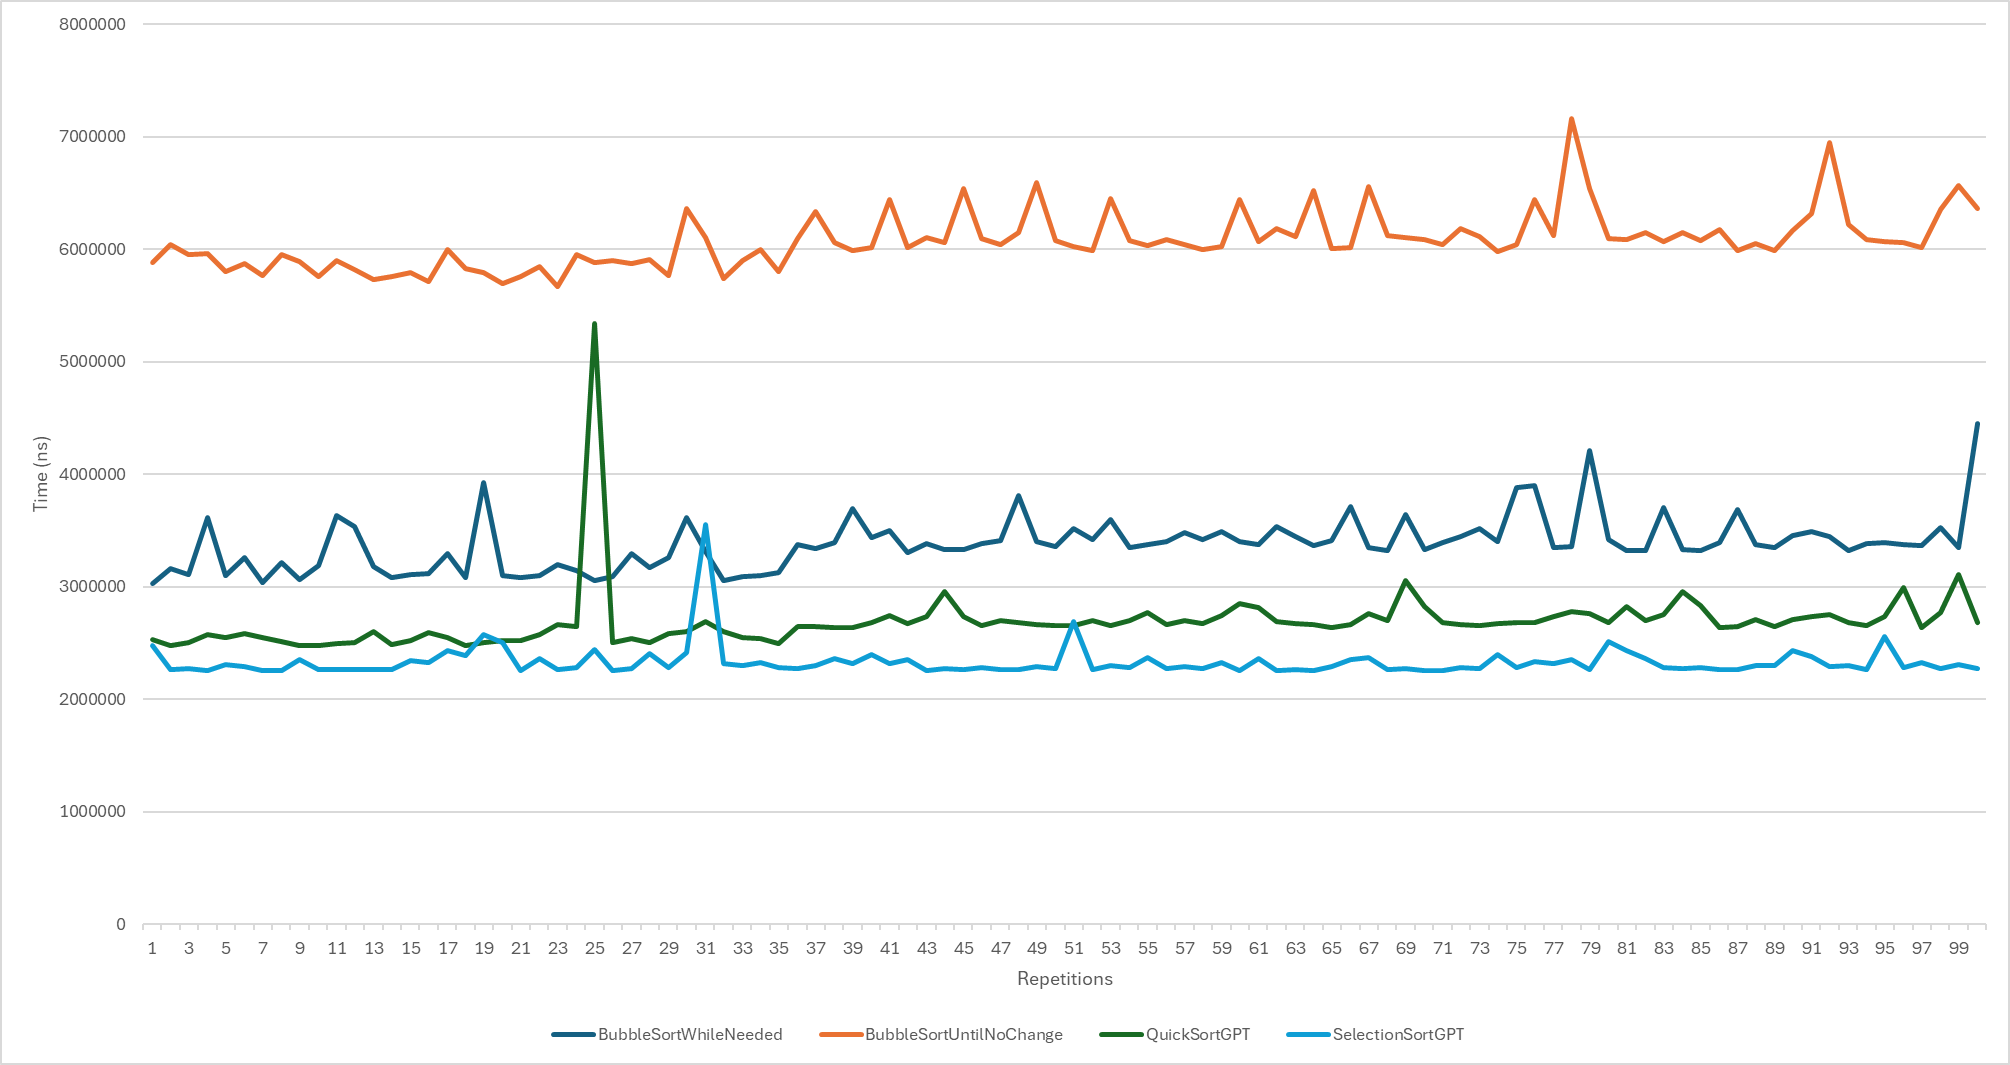
\includegraphics[width=0.7\linewidth]{char_1000_reverse_sorted.png}
        \caption{Results of sorting a reverse sorted array of size 1000 made from char}
        \label{fig:char_1000_reverse_sorted}
    \end{figure}
    
    \begin{figure}[!h]
        \centering
        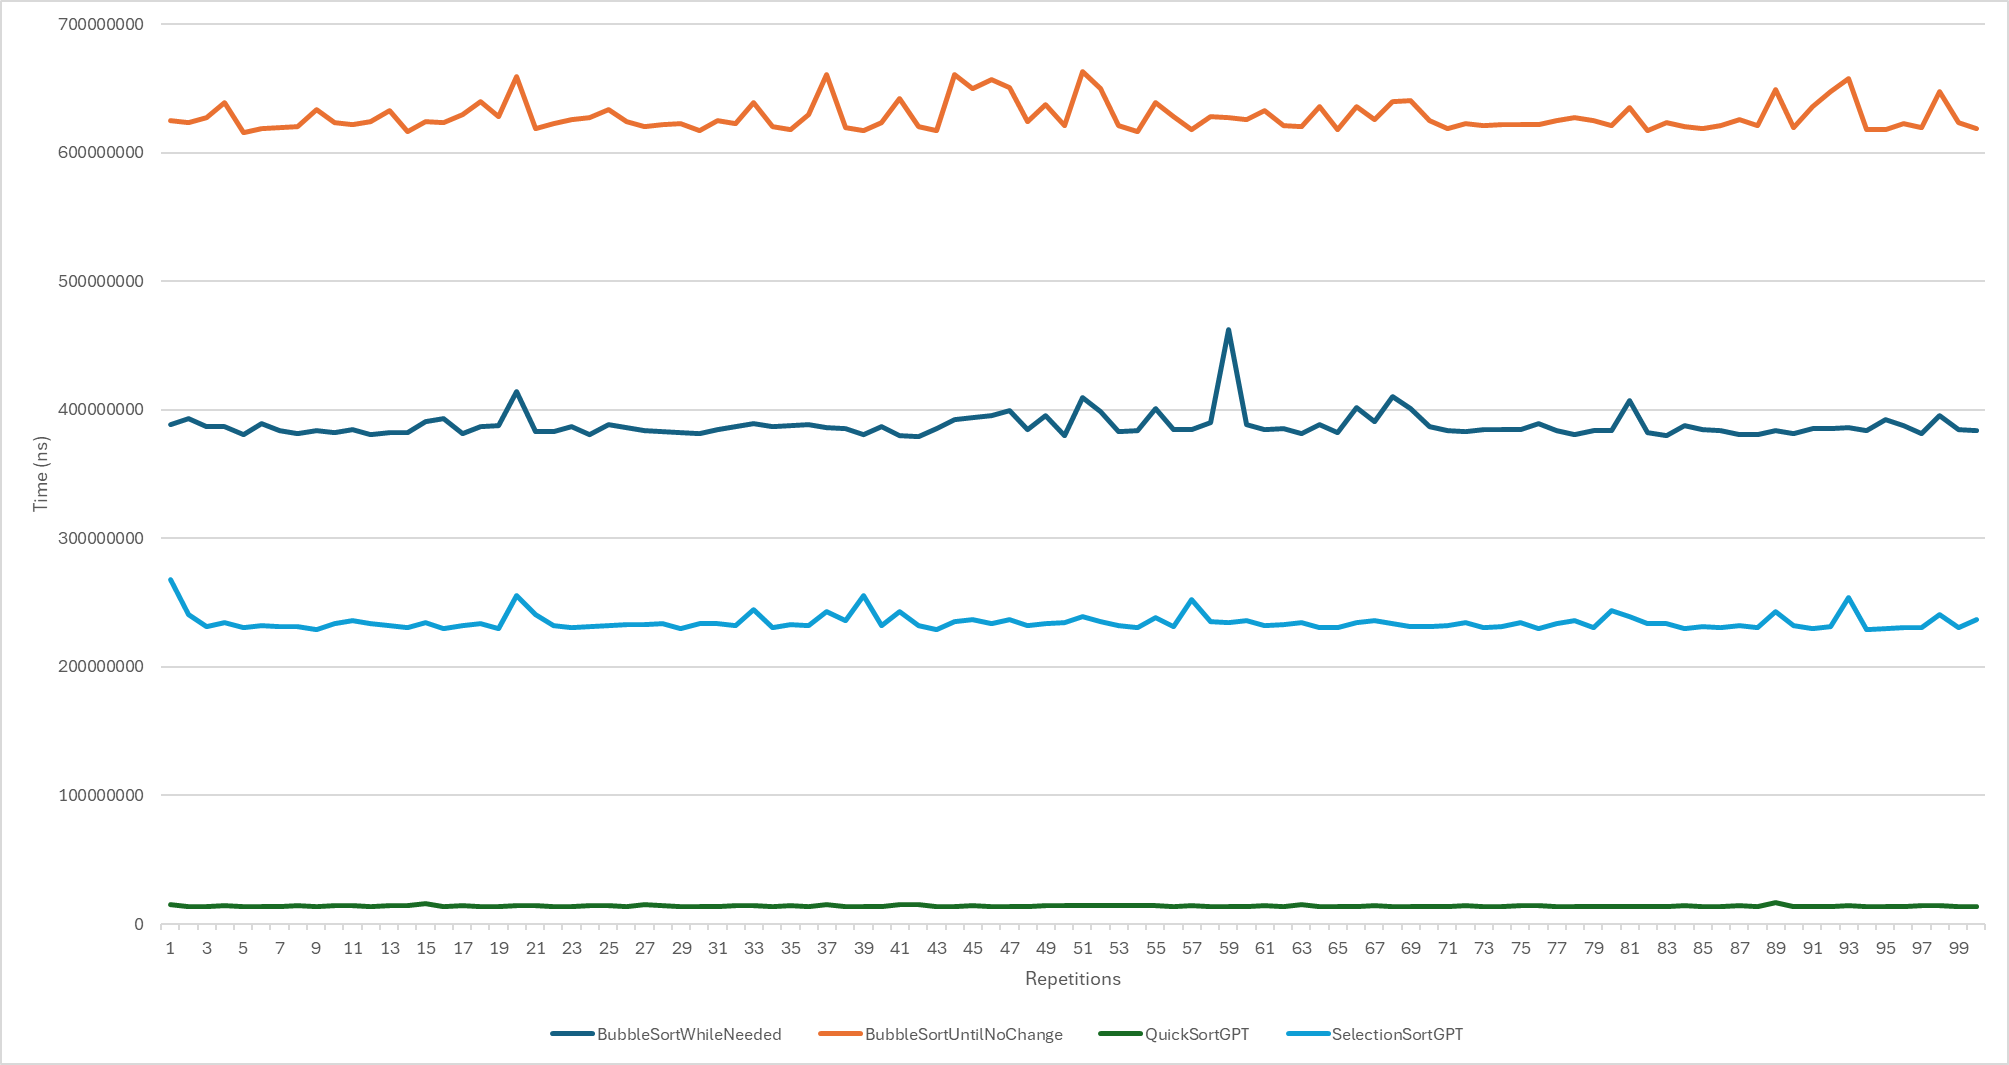
\includegraphics[width=0.7\linewidth]{char_10000_random.png}
        \caption{Results of sorting a randomly filled array of size 10000 made from char}
        \label{fig:char_10000_random}
    \end{figure}
    
    \begin{figure}[!h]
        \centering
        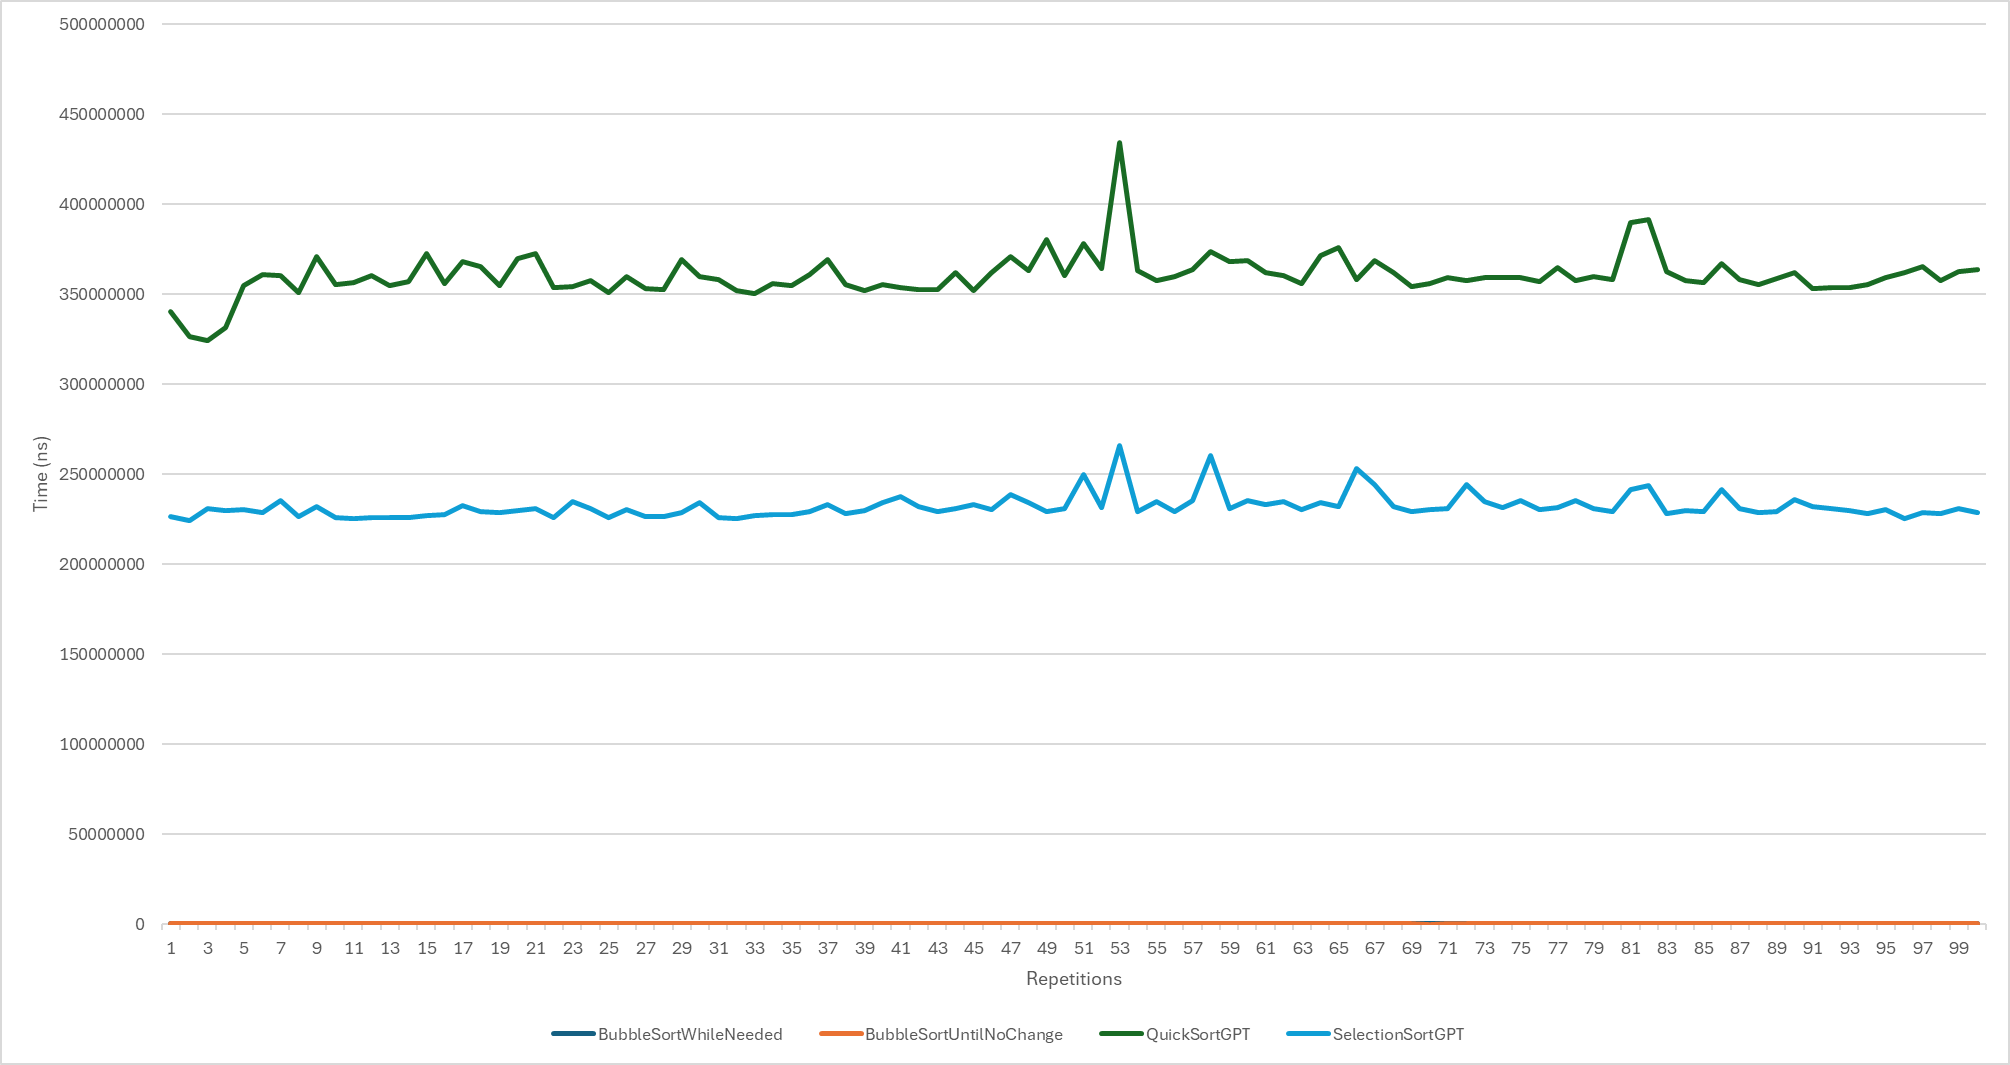
\includegraphics[width=0.7\linewidth]{char_10000_sorted.png}
        \caption{Results of sorting a sorted array of size 10000 made from char}
        \label{fig:char_10000_sorted}
    \end{figure}
    
    \begin{figure}[!h]
        \centering
        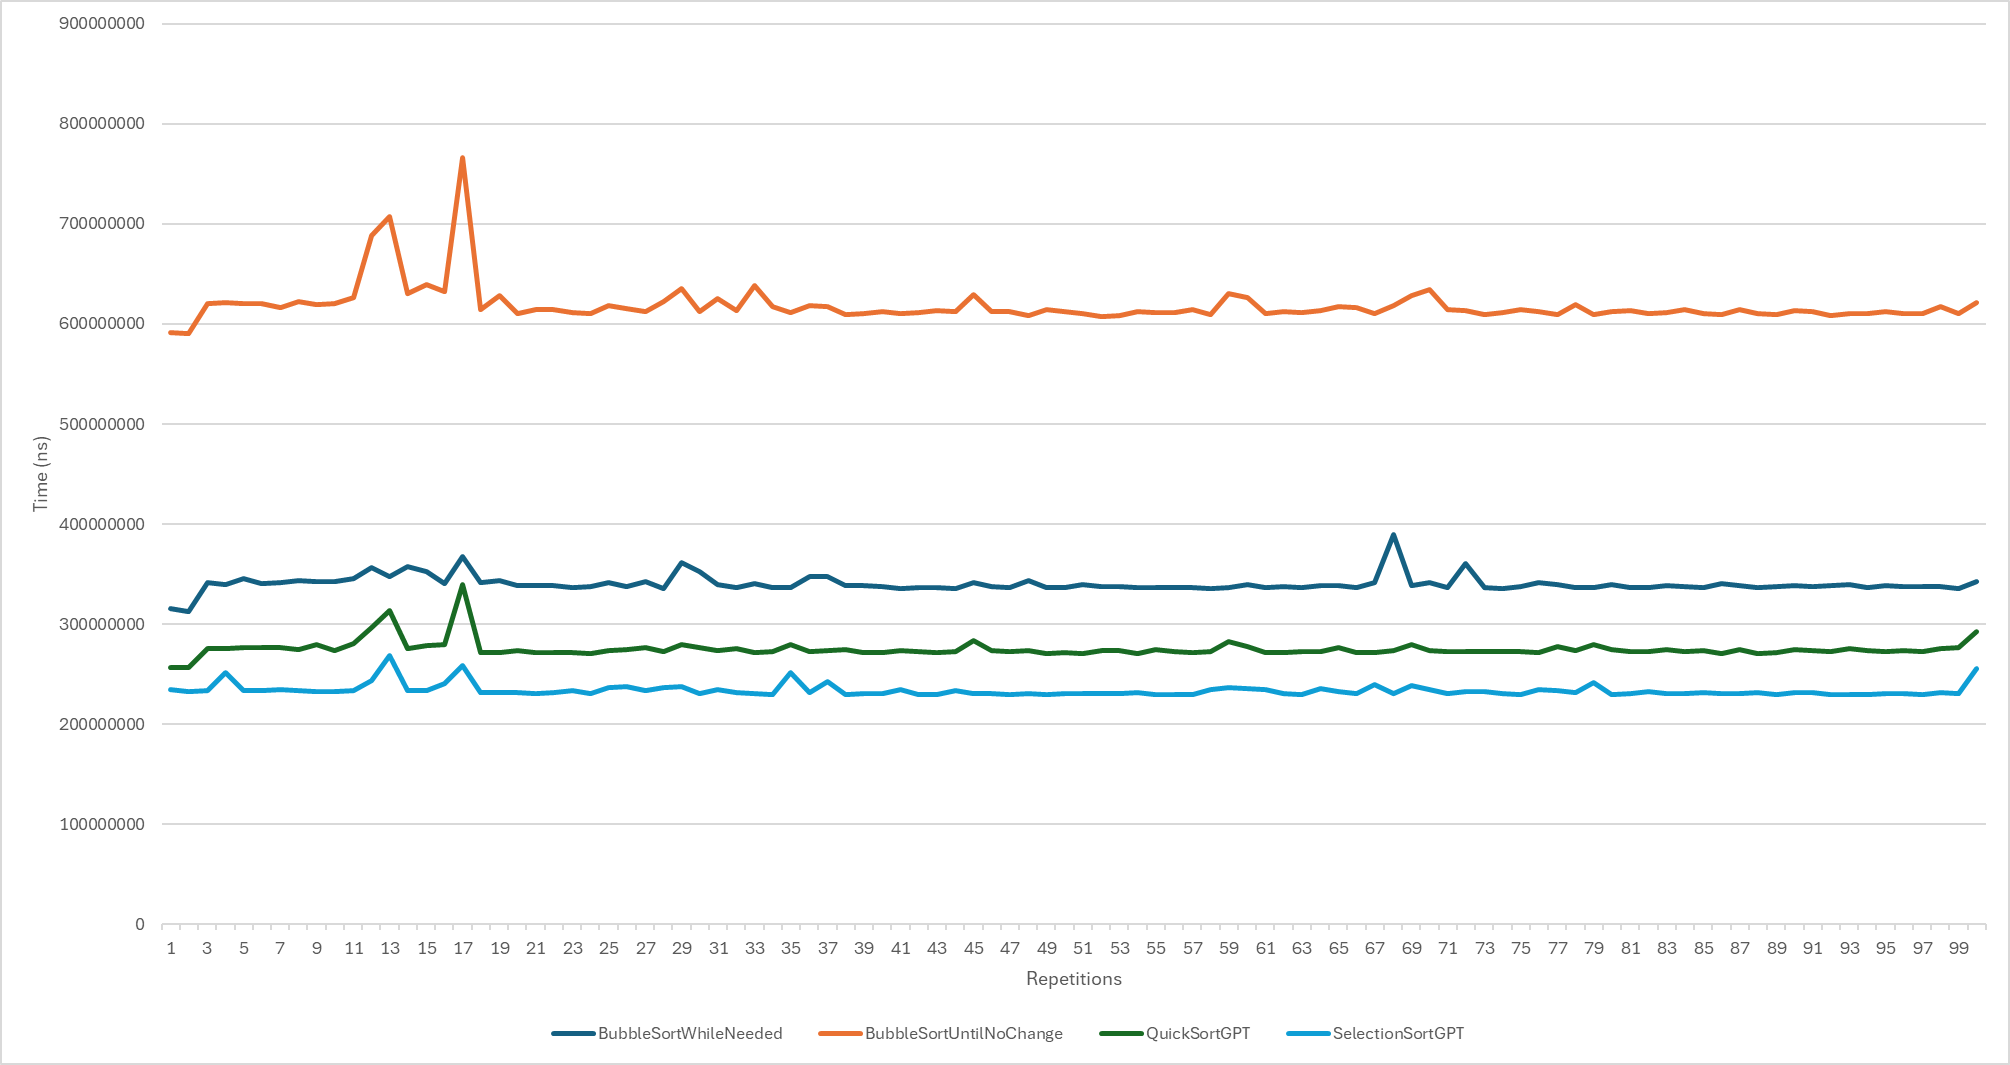
\includegraphics[width=0.7\linewidth]{char_10000_reverse_sorted.png}
        \caption{Results of sorting a reverse sorted array of size 10000 made from char}
        \label{fig:char_10000_reverse_sorted}
    \end{figure}

    %bool

     \begin{figure}[!h]
        \centering
        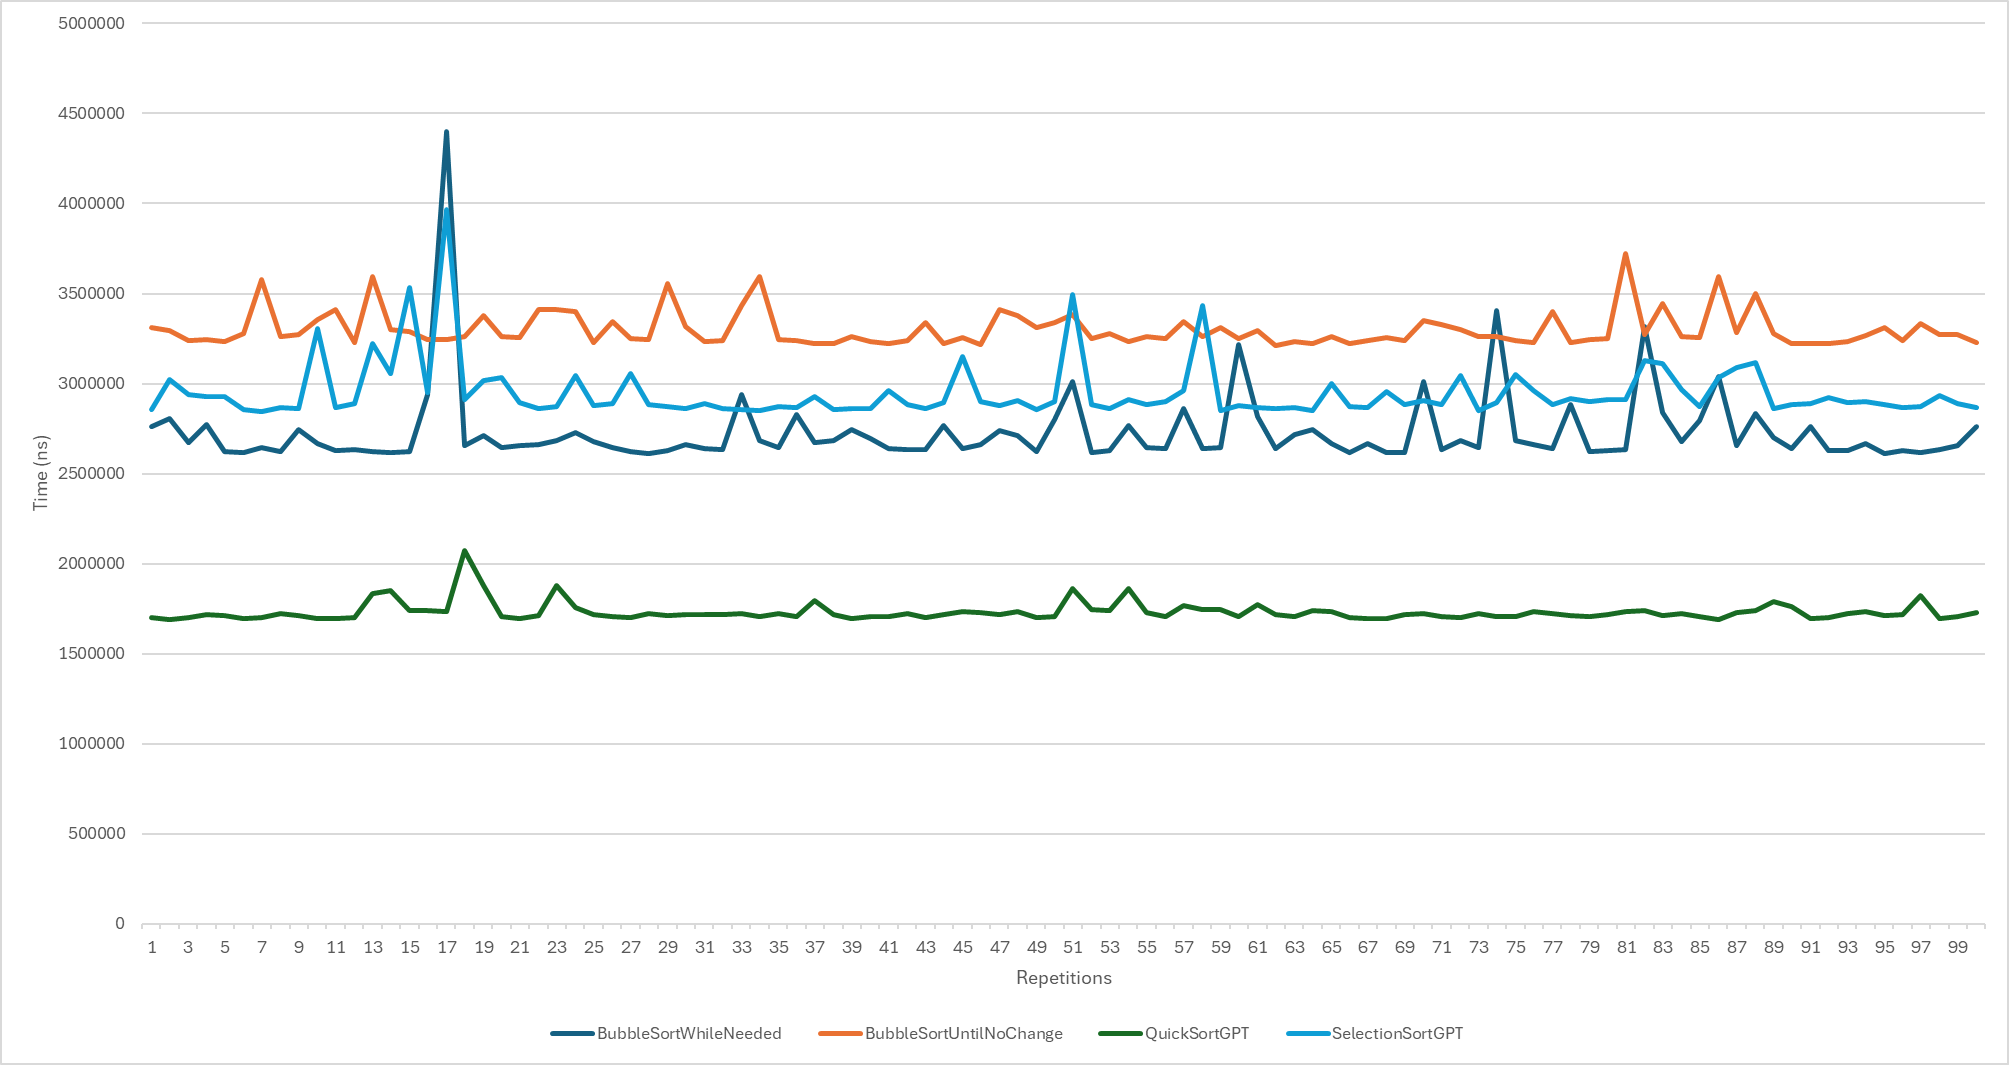
\includegraphics[width=0.7\linewidth]{bool_1000_random.png}
        \caption{Results of sorting a randomly filled array of size 1000 made from bool}
        \label{fig:bool_1000_random}
    \end{figure}
    
    \begin{figure}[!h]
        \centering
        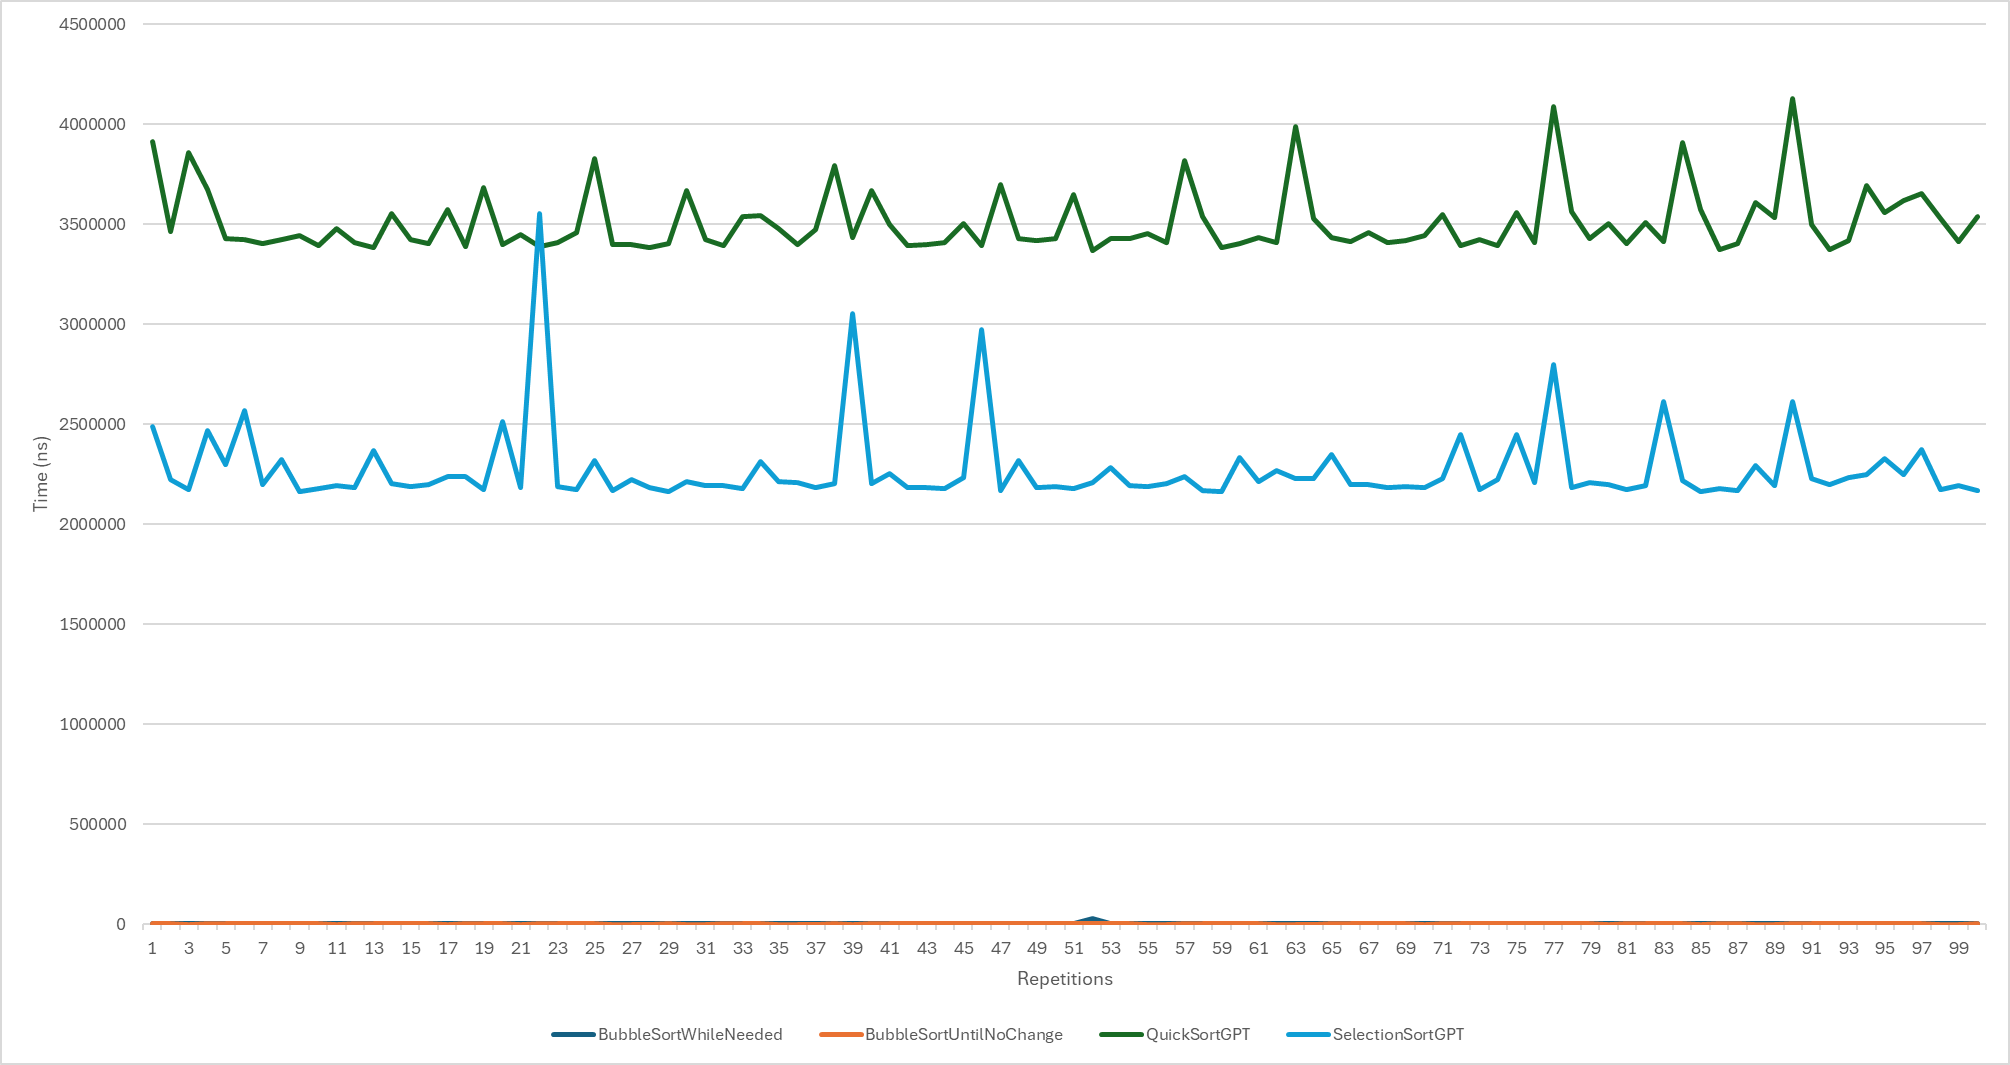
\includegraphics[width=0.7\linewidth]{bool_1000_sorted.png}
        \caption{Results of sorting a sorted array of size 1000 made from bool}
        \label{fig:bool_1000_sorted}
    \end{figure}
    
    \begin{figure}[!h]
        \centering
        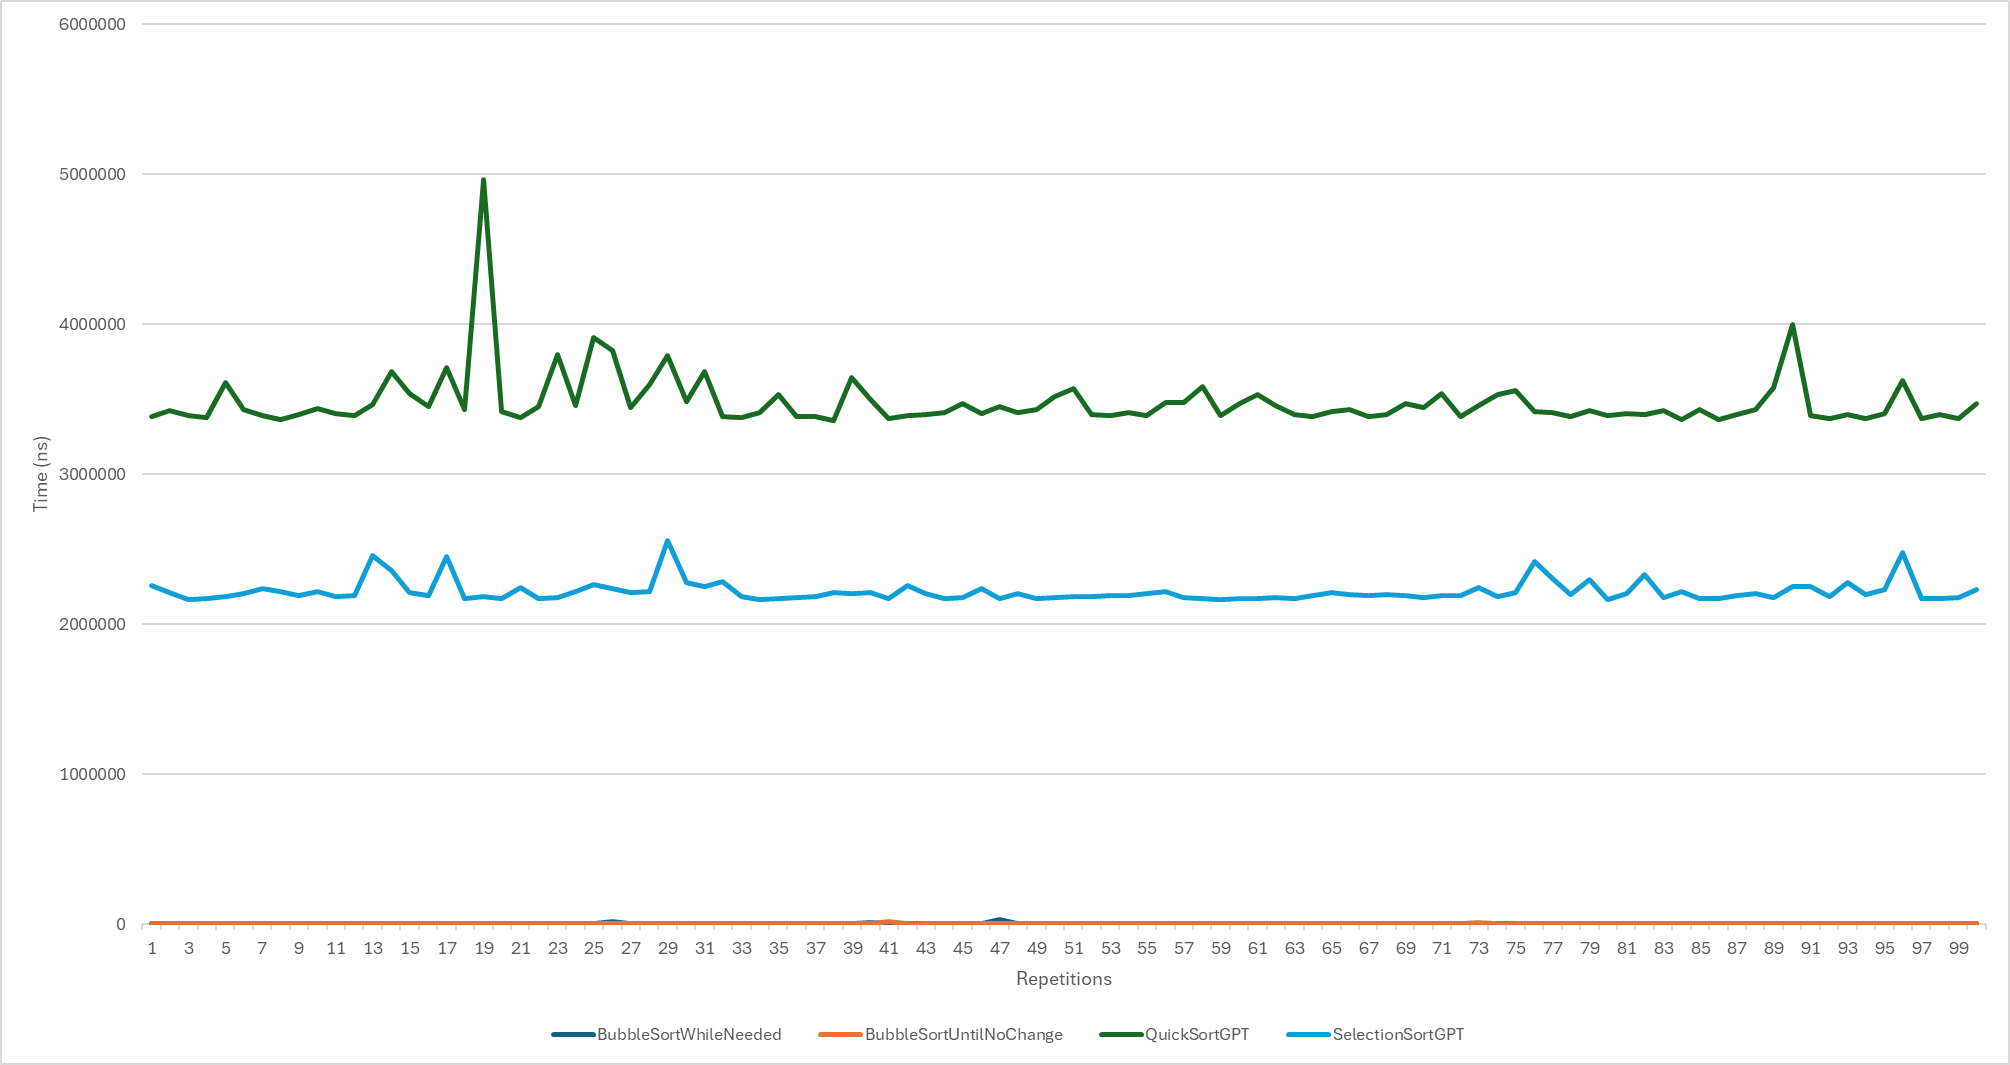
\includegraphics[width=0.7\linewidth]{bool_1000_reverse_sorted.png}
        \caption{Results of sorting a reverse sorted array of size 1000 made from bool}
        \label{fig:bool_1000_reverse_sorted}
    \end{figure}
    
    \begin{figure}[!h]
        \centering
        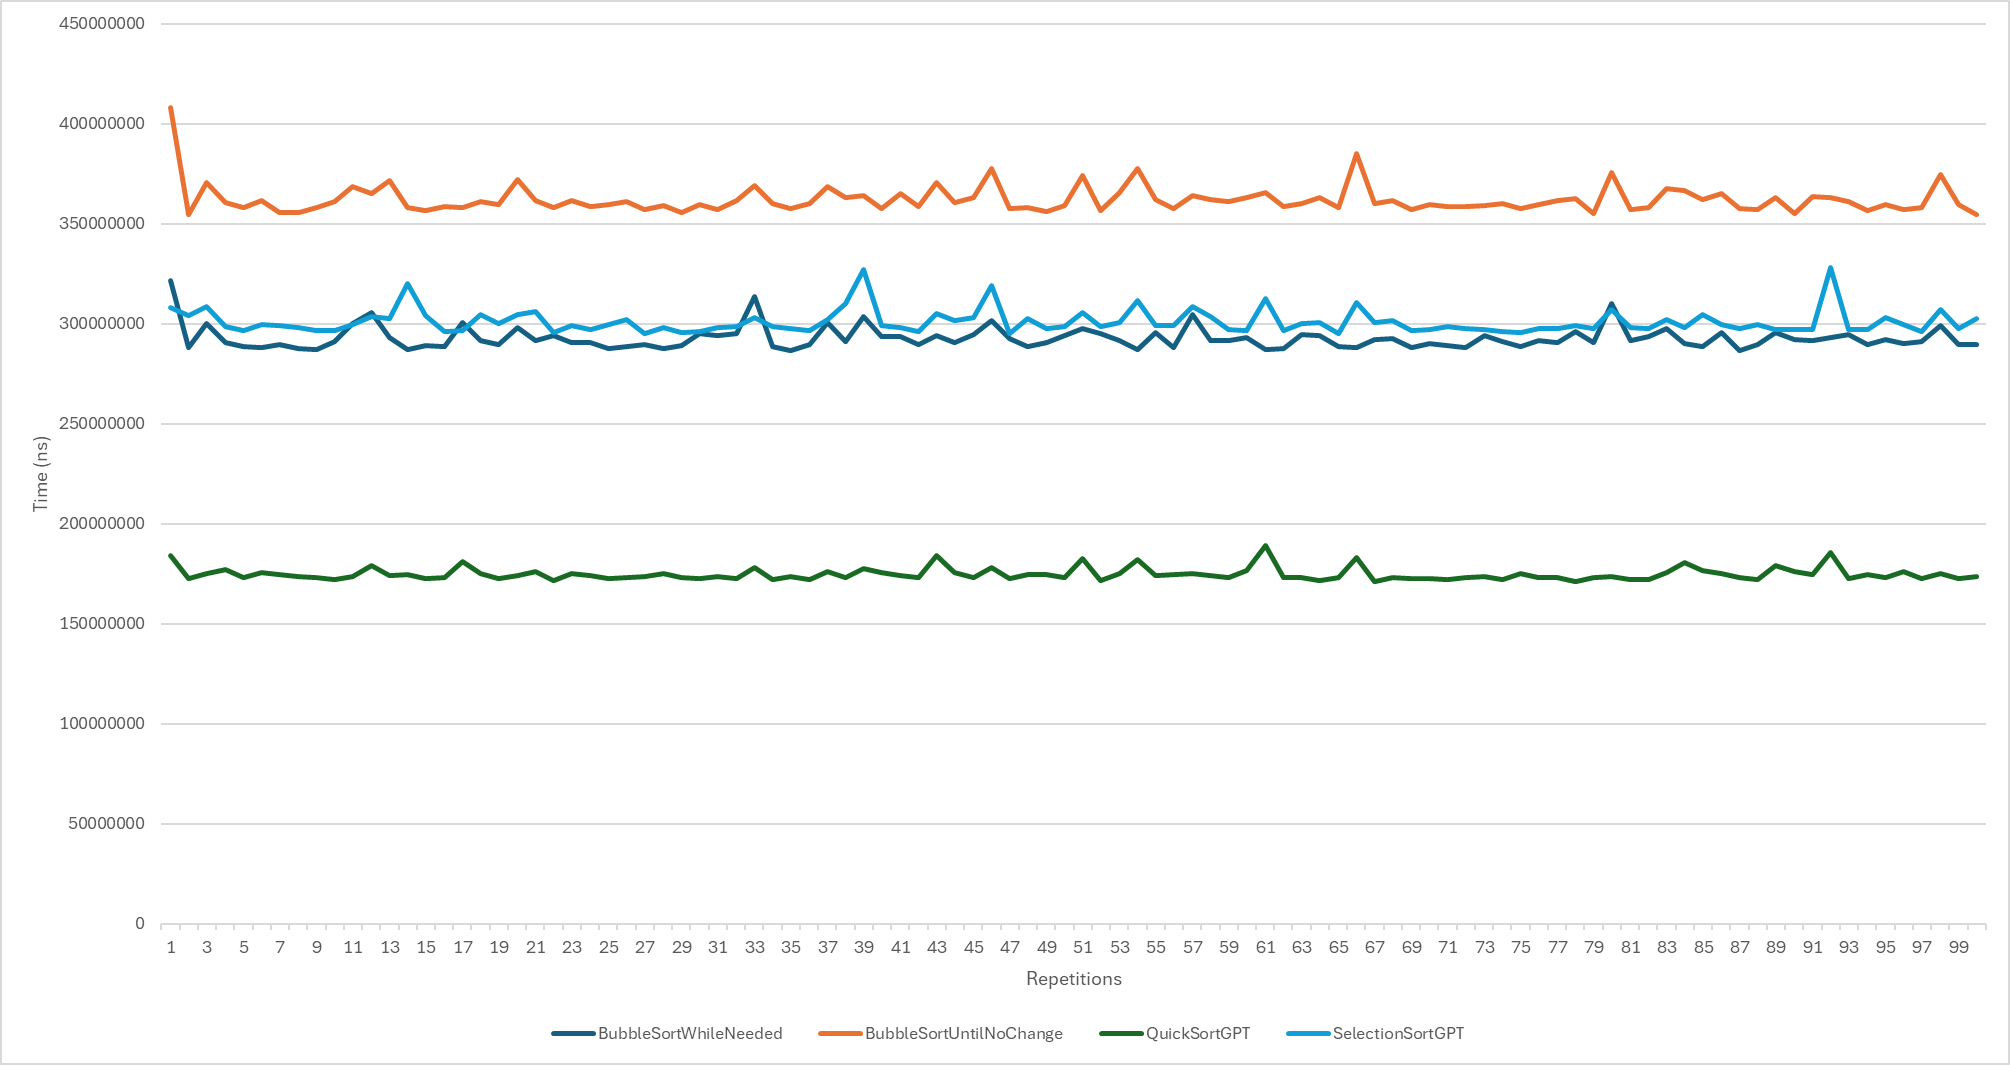
\includegraphics[width=0.7\linewidth]{bool_10000_random.png}
        \caption{Results of sorting a randomly filled array of size 10000 made from bool}
        \label{fig:bool_10000_random}
    \end{figure}
    
    \begin{figure}[!h]
        \centering
        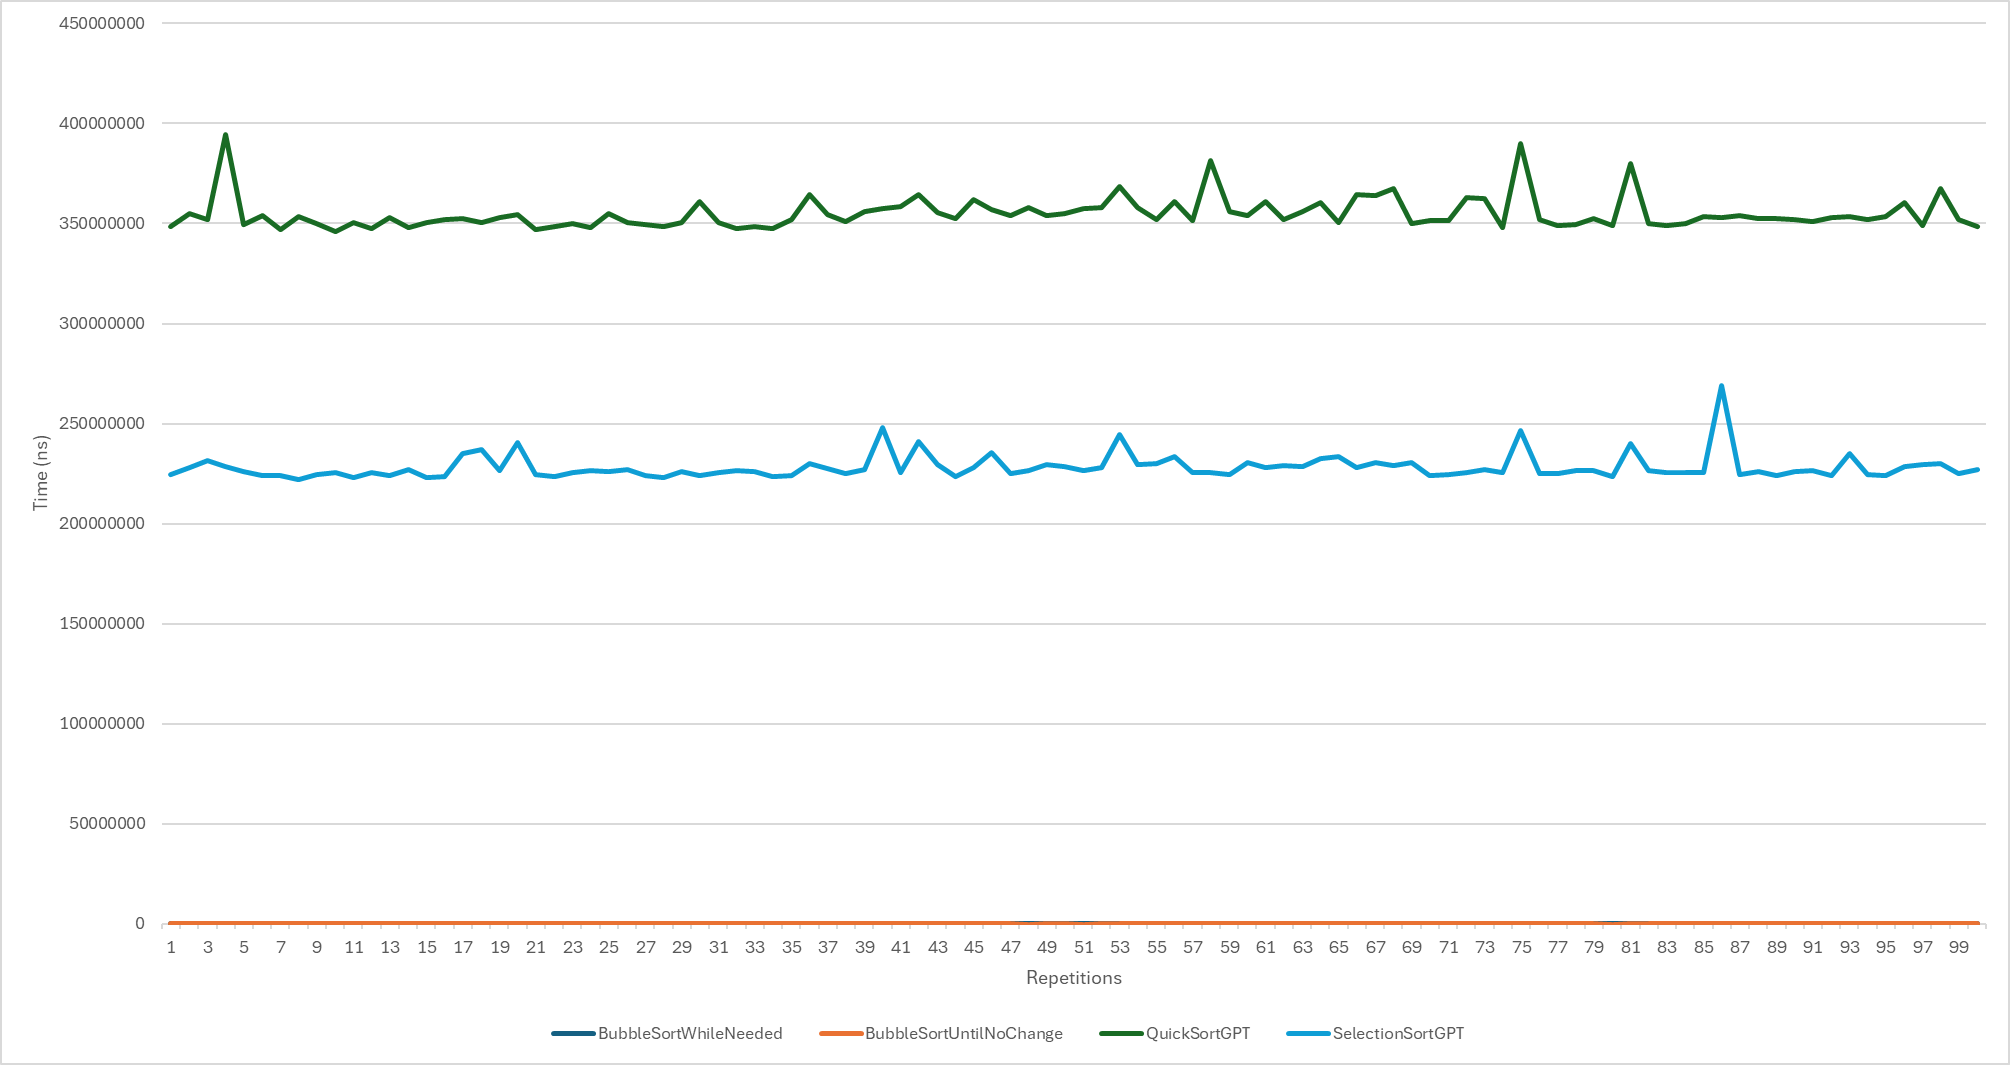
\includegraphics[width=0.7\linewidth]{bool_10000_sorted.png}
        \caption{Results of sorting a sorted array of size 10000 made from bool}
        \label{fig:bool_10000_sorted}
    \end{figure}
    
    \begin{figure}[!h]
        \centering
        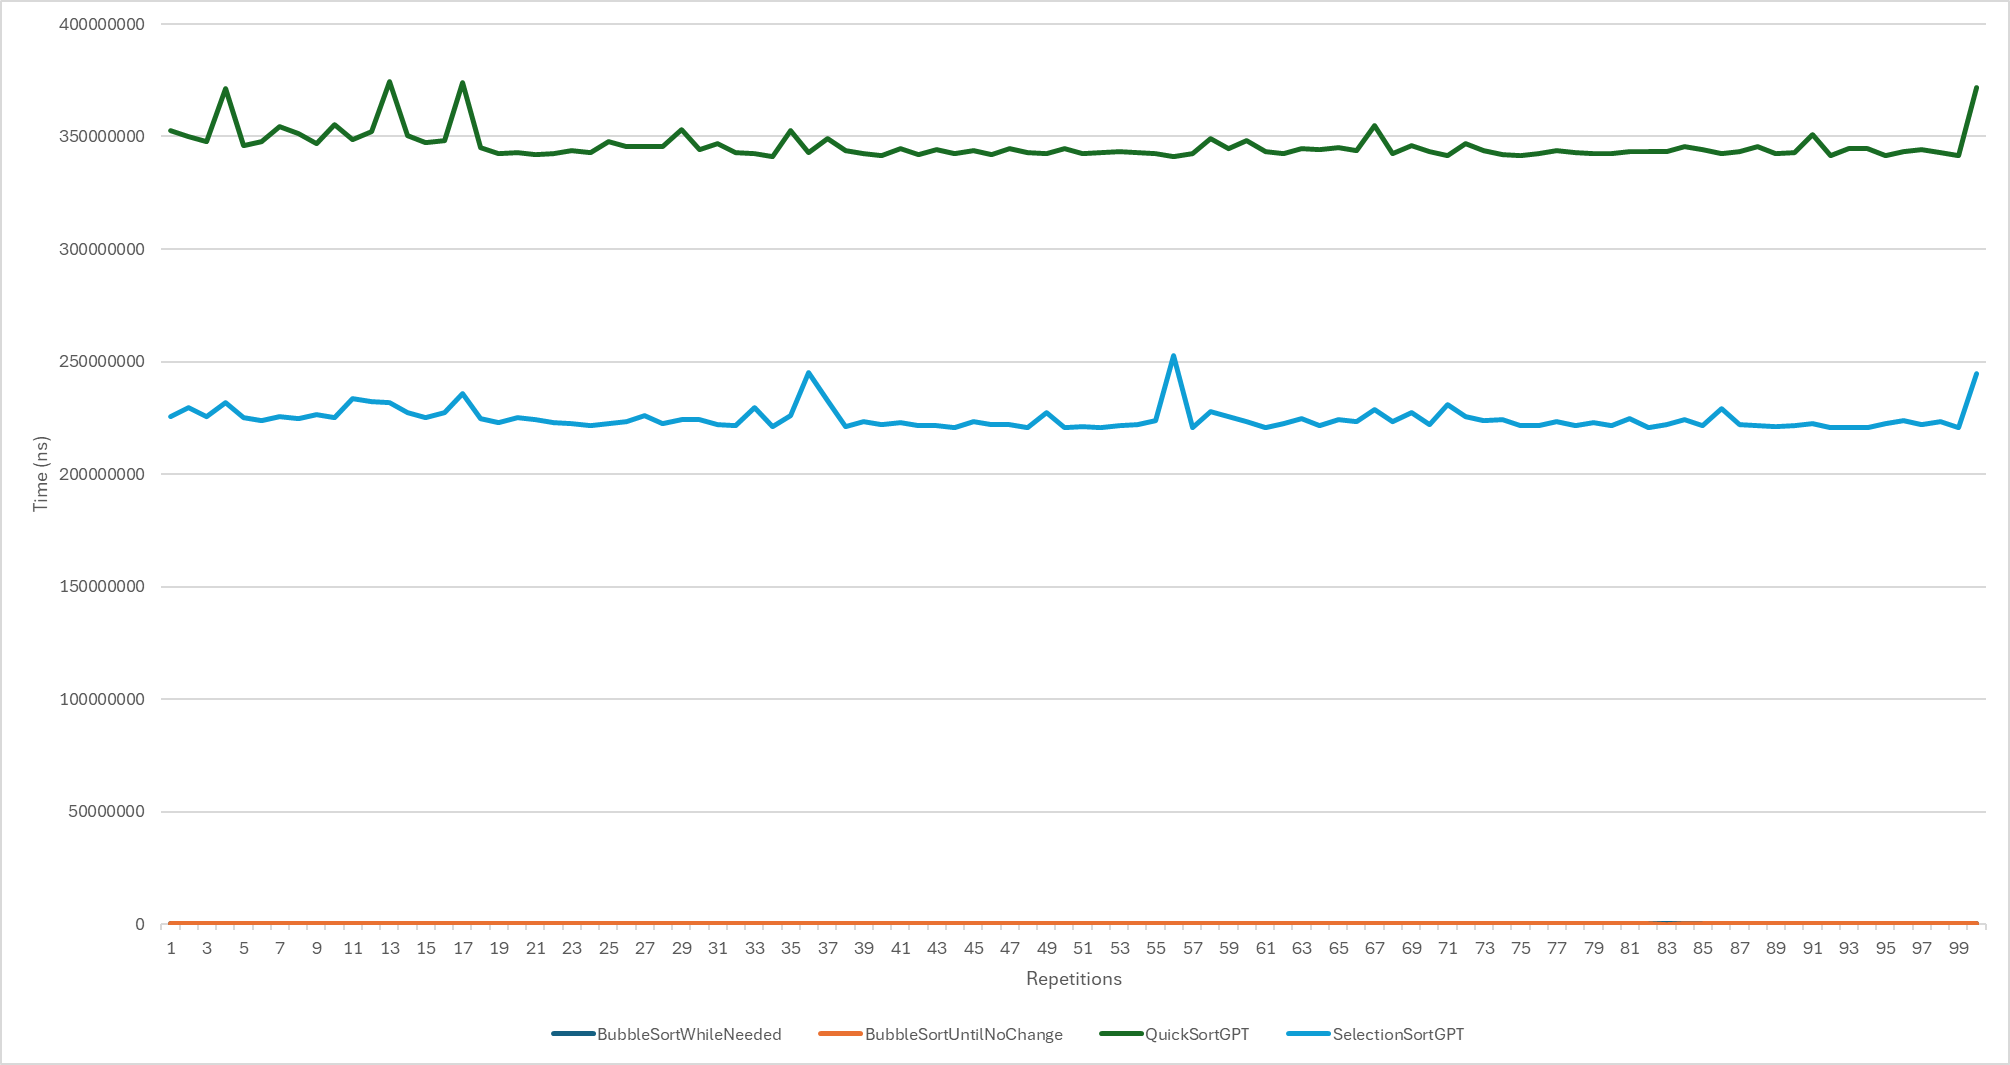
\includegraphics[width=0.7\linewidth]{bool_10000_reverse_sorted.png}
        \caption{Results of sorting a reverse sorted array of size 10000 made from bool}
        \label{fig:bool_10000_reverse_sorted}
    \end{figure}
    
    \clearpage

\end{document}